\chapter{A Quick Overview of Matching}

This chapter will give a global overview of the tools, and the
concept they use.  This chapter is restricted to matching,
an overview of orientation is given in chapter~\ref{Intro:QuickApero}.
It is not a formal or complete description,  this
will be done in further chapters; here there are essentially examples
and comments.

\label{Intro:QuickR}

%-------------------------------------------------------------------
%-------------------------------------------------------------------
%-------------------------------------------------------------------

\section{Installing the Tools}

    % - - - - - - - - - - - - - - - - - - - - -

\subsection{svn Extraction}

All that you need to install the tools and run the example can be found on the site 
{\tt http://www.micmac.ign.fr/}. Clik on {\tt T\'el\'echargement} to go to the 
download page. To have an up to date version, you will need to install
the {\tt subversion} tools.  To get the {\tt micmac}  softwares, type:

{\tt svn co http://www.micmac.ign.fr/svn/micmac/trunk micmac }

    % - - - - - - - - - - - - - - - - - - - - -

\subsection{Compilation}

The {\tt Readme.txt} contains the list of instructions necessary to install
the sofware. As they are distributed in source code, it may be a bit long (15 min
on a mono processor computer)
as it will require full compilation.

Follow exactly the directive of {\tt Readme.txt}, including directory creation
and the required {\tt touch} actions. {\tt touch}  is necessary  to
break some tricky circular dependencies in the {\tt Makefile}.

After the installation, there should exist on {\tt /usr/local/bin/} a file
{\tt MicMacConfig.xml}, that describes some installation configuration,
it should look like :

\label{Mic:File:Config}

\begin{verbatim}
<?xml version="1.0" ?>
<MicMacConfiguration>
     <DirInstall>/home/mpd/micmac/</DirInstall>
     <NbProcess>2</NbProcess>
</MicMacConfiguration>
\end{verbatim}


    % - - - - - - - - - - - - - - - - - - - - -

\subsection{Some Important Directories}

Starting from the {\tt micmac} directory, there are some important directories
to know:

\begin{itemize}
   \item {\tt include/XML\_GEN/}, where you will find the formal {\tt XML} specification that will
         be described in chapter~\ref{Mic:Tree:Match};

   \item {\tt Documentation/DocMicMac/}, where you will find this documentation and others
        documents related to these tools;

   \item {\tt bin/}, will contain the executable command generated  after the different {\tt make};
\end{itemize}


If you are in software development and interested to take a look at the code, 
here are others directories:


\begin{itemize}
   \item {\tt src}, all the \CPP code needed to generate the \ELISE lib, this is a general image library
         I developped before MicMac, all the tools are using this lib for basic manipulation;

   \item {\tt include/}, all the header files  needed by src files for \ELISE ;

   \item {\tt applis}, all the \CPP code needed to generate  the different tools;  main tools, as
         {\tt MicMac} or {\tt Apero} have their own sub-directories (for ex, {\tt applis/Apero/}),
         when auxiliary tools are contained in a single file (for example {\tt applis/uti\_phgrm/Nuage2Ply.cpp});

   \item {\tt objets/}  will contain the results of compilation.

\end{itemize}



    % - - - - - - - - - - - - - - - - - - - - -

\subsection{Installing the Examples}

You can download several examples (many of them are obsolete ...) and the interface of
Isabelle Clery, by typing:

{\tt svn co http://www.micmac.ign.fr/svn/micmac\_data/trunk micmac\_data}

However, it may be a bit long, depending of the bandwise. If you do not need
the interface for now and only want the example of this documentation, you can type :

{\tt svn co http://www.micmac.ign.fr/svn/micmac\_data/trunk/ExempleDoc/ micmac\_data/ExempleDoc/}




% - - - - - - - - - - - - - - - - - - - - -

\subsection{Verification and Global Vision of the Main Tools}

\label{SHEL:TEST:BOUDHA}

Once the installation is completed \footnote{tools are built and you got data
on {\tt ExempleDoc}}, go into the micmac directory,
and take a look at the file {\tt Test0Boudha.sh}. It contains
$3$ command lines:

{\scriptsize
\begin{verbatim}
bin/Tapioca MulScale ../micmac_data/ExempleDoc/Boudha/IMG_[0-9]{4}.tif 300 -1 ExpTxt=1
bin/Apero  ../micmac_data/ExempleDoc/Boudha/Apero-5.xml
bin/MICMAC  ../micmac_data/ExempleDoc/Boudha/Param-6-Ter.xml
\end{verbatim}
}

This is a typical simple execution of the pipeline to build $3D$ models from images:

\begin{itemize}
    \item the first line {\tt bin/Tapioca} is the command line for generating tie points
          from a set of images; this tool in described in~\ref{Tapioca};

    \item the second line {\tt bin/Apero} is the command line for generating orientations;
           it is described in~\ref{Intro:QuickApero};


    \item the third line {\tt bin/MICMAC} is the command line for generating dense
          matching from oriented images; it is decribed in this chapter;
\end{itemize}



Practically, the ordering of different phases will always be: %1- Tie Points 2- Orientation 3- Dense Matching

\begin{enumerate}
	\item Tie Points
	\item Orientation
	\item Dense Matching.
\end{enumerate}

However, in this quick overview, we present it in the reverse
order because it is dense matching that justifies orientation, and it is orientation
that justifies tie points.

Being still in the micmac directory, type:

\begin{center}
\begin{verbatim}
            source Test0Boudha.sh 
\end{verbatim}
\end{center}

You will see a lot of text on the terminal. %console.  
Do not stop the process, it will
produce data, that will be used in the rest of the examples.
If everything is correctly installed, it will be over after $15$ minutes
(or less, according to your computer). Check the directory:

\begin{center}
\begin{verbatim}
            micmac_data/ExempleDoc/Boudha/MEC-6-Im/
\end{verbatim}
\end{center}

You must have $3$ files  having a {\tt .ply} extension. You can take a look at these files
using a free software such as {\tt MeshLab}.

%-------------------------------------------------------------------
%-------------------------------------------------------------------
%-------------------------------------------------------------------



%-------------------------------------------------------------------
%-------------------------------------------------------------------
%-------------------------------------------------------------------

\section{A MicMac Example Using Simplest Parametrization}

All the data needed in the following part are in the directory 
{\tt micmac\_data/ExempleDoc/Boudha/}.


\subsection{Epipolar Geometry}

For this first set of examples, to make it simple, we will treat
a pair of images that have been resampled in epipolar geometry.
These images are {\tt Epi-Left.tif} and {\tt Epi-Right.tif}.
The figure~\ref{FIG:EPIP} shows a quick wiew of these two images.


\begin{figure}
\hspace{10 mm}
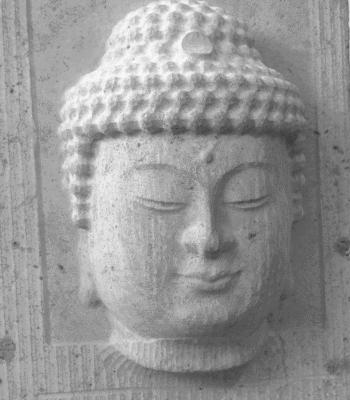
\includegraphics[height=60mm]{FIGS/Boudhas/Epi-Left.jpg}
\hspace{10 mm}
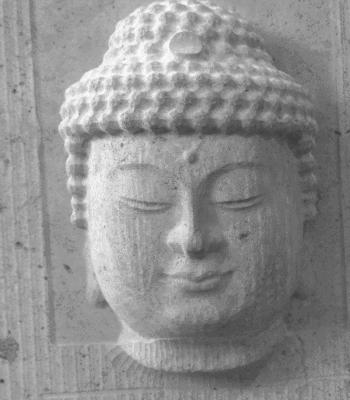
\includegraphics[height=60mm]{FIGS/Boudhas/Epi-Right.jpg}
\caption{The pair of epipolar images used in these examples}
\label{FIG:EPIP}
\end{figure}


According to the definition of epipolar, for each point $x,y$ of {\tt Epi-Left.tif} its
homologous point, in  image {\tt Epi-Right.tif}, is located on the same line, so at
position $x',y$.  The aim of epipolar matching is, given $x,y$,  compute the
disparity $d(x,y)=x'-x$ so that $x+d(x,y),y$ is homologous of  $x,y$.

Obviously, epipolar geometry is not very interesting in modern
photogrammetry, however it will allow to separate in this introduction the 
paramaters related to  matching  from parameters related to geometry.



MicMac uses (almost always) the normalized cross-correlation coefficient
as a similarity measurement. See the chapter~\ref{CHAP:COREL} if you
forgot the meaning of this coefficient.

One of the simplest matching algorithm for computing a disparity map is
the folowing:

\begin{itemize}
    \item let $Sz$ be the size of correlation window, $D$ be the size of the
          disparity interval, and $Cor(x_1,y_1,x_2,y_2,Sz)$ be the normalized
          cross correlation between two windows of size $Sz$, centered on $x_1,y_1$
           and $x_2,y_2$;

    \item set $d(x,y) = ArgMax_{d\in[-D,D]} Corr(x,y,x+d,y,Sz)$;
\end{itemize}


\subsection{Analyzing Matching Parameters}

{\scriptsize
\setlength{\columnseprule}{0.5pt}
\begin{multicols}{2}
\begin{verbatim}
<!--
   The simplest MicMac example
-->

<ParamMICMAC>
  <Section\_PriseDeVue >
     <GeomImages> eGeomImage\_EpipolairePure </GeomImages>
     <Images >
          <Im1> Epi-Left.tif </Im1>
          <Im2> Epi-Right.tif </Im2>
     </Images>
  </Section\_PriseDeVue>

  <Section\_Terrain>  
      <IntervParalaxe>
             <Px1IncCalc>   50.0  </Px1IncCalc>
       </IntervParalaxe>
  </Section\_Terrain>
  <Section\_MEC >

	 <EtapeMEC>
             <DeZoom >  -1                      </DeZoom>
             <SzW >      1             </SzW>
             <AlgoRegul>    eAlgoMaxOfScore    </AlgoRegul>

             <Px1Pas>        1  </Px1Pas>

             <!-- Unused but mandatory -->
	     <Px1DilatAlti>  0    </Px1DilatAlti>
             <Px1DilatPlani> 0    </Px1DilatPlani>
	     <Px1Regul>  0    </Px1Regul>
        </EtapeMEC>
	     

        <EtapeMEC> <DeZoom >  1  </DeZoom> </EtapeMEC>

  </Section\_MEC>

  <Section\_Results >
        <GeomMNT> eGeomPxBiDim  </GeomMNT> 
  </Section\_Results>

  <Section\_WorkSpace >
        <WorkDir >  ThisDir </WorkDir> 
        <TmpMEC>  MEC-0-EPI/  </TmpMEC>
        <TmpResult>  MEC-0-EPI/  </TmpResult>
        <TmpPyr>    Pyram-Epi/  </TmpPyr>
  </Section\_WorkSpace>


<Section\_Vrac> </Section\_Vrac>

</ParamMICMAC>
\end{verbatim}
\end{multicols}
}

The file {\tt Param-0-Epi.xml} contains parameters for MicMac  to execute
the previous simple algorithm. Some comments:

\begin{itemize}
   \item  the most encompassing tag is {\tt ParamMICMAC}\footnote{= shooting section },
   		 there must be only one;
          {\tt MicMac} loads and interprets all the information contained in this tag;

   \item the first level tag {\tt Section\_PriseDeVue}\footnote{= shooting section }
         contains parameters about
         image acquisition,  the name of images are in tags 
         {\tt Im1} and {\tt Im2} and the tag {\tt GeomImages} whose value
         {\tt eGeomImage\_EpipolairePure} means that the image have been sampled
         in epipolar geometry;

    \item the tag {\tt Section\_Terrain} \footnote{= Ground section} contains information
          about the terrain, in other geometry it may be the interval of $Z$ and the desired
          footprint; here, we are in epipolar geometry, so the "terrain" is just the image space,
          $x$ and $y$ are pixel of master image and the only required information  is the disparity 
           interval specified in the tag {\tt IntervParalaxe};

 
    \item the tag {\tt Section\_MEC} \footnote{= Mise En Correspondance = Matching} contains the
          information relative to the algorithmic aspect; it is detailed below;

    \item  the tag {\tt Section\_Results} contains the information necessary to generate the  desired results; here it is semantically
           empty, the value {\tt eGeomPxBiDim} of {\tt GeomMNT} being mandatory in the epipolar case;

    \item the tag {\tt Section\_WorkSpace} contains the information for files organisation;
           the value {\tt ThisDir} of tag {\tt WorkDir} means that all the names of files are
           relative to the directory where the parameter file is located.

\end{itemize}


The  {\tt Section\_MEC} can be very complex; MicMac has a multi-resolution approach in which
several phases of matching are piped, for each step all the algorithmic parameters can be changed if necessary. 
However, generally this is not desired, so to limit the complexity,
when the parameters are mainly constant for all phases,  MicMac has the following mechanism:


\begin{itemize}
    \item the first {\tt Section\_MEC}  is not executed, it conventionnaly sets the default
          parameters of all the following  {\tt Section\_MEC}, it is mandatory that the 
          tag {\tt DeZoom}, fixing the resolution, has the value $-1$ for this first step;


    \item the default parameters set in this example are:

\begin{itemize}
         \item {\tt SzW} sets the size of the correlation window, the value $1$
               means in fact $[-1,1]x[-1,1]$;

          \item {\tt AlgoRegul} specifies the possible regularization algorithm,  in this
                simplest example, the value {\tt eAlgoMaxOfScore} means that there is
                no regularization (i.e. compute arg-max);

          \item {\tt Px1Pas} specifies the quantization step of  the disparity map;
                here, the value $1$ means in fact that  only the integer disparity is tested;

          \item all the other tags are mandatory for internal reason but they have no
                meaning here;
\end{itemize}

    \item in this example, there is only one phase, and as all the interesting parameters
          have been set in the default phase, it contains only the resolution parameter
          {\tt DeZoom}, here we work at full resolution, so $DeZoom=1$.

\end{itemize}



\subsection{Running the Program}

Now, type the following command:

{\tt
bin/MICMAC ~/micmac\_data/ExempleDoc/Boudha/Param-0-Epi.xml 
}

The terminal should print a lot of idiot messages like:

{\scriptsize
\begin{verbatim}
<< Make Masq Resol 1 /home/mpd/micmac_data/ExempleDoc/Boudha/MEC-0-EPI/Masq_LeChantier_DeZoom1.tif
>>  Done Masq Resol 1 /home/mpd/micmac_data/ExempleDoc/Boudha/MEC-0-EPI/Masq_LeChantier_DeZoom1.tif
>> Done Masque for /home/mpd/micmac_data/ExempleDoc/Boudha/MEC-0-EPI/Masq_LeChantier_DeZoom1.tif
....
<< Make Masque for /home/mpd/micmac_data/ExempleDoc/Boudha/MEC-0-EPI/Masq_LeChantier_DeZoom64.tif
>> Done Masque for /home/mpd/micmac_data/ExempleDoc/Boudha/MEC-0-EPI/Masq_LeChantier_DeZoom64.tif
....
<< Make Pyram for /home/mpd/micmac_data/ExempleDoc/Boudha/Epi-Right.tif
>> Done Pyram for /home/mpd/micmac_data/ExempleDoc/Boudha/Epi-Right.tif
....
<< Make Pyram for /home/mpd/micmac_data/ExempleDoc/Boudha/Pyram-Epi/Epi-Left.tifDeZoom64.tif
>> Done Pyram for /home/mpd/micmac_data/ExempleDoc/Boudha/Pyram-Epi/Epi-Left.tifDeZoom64.tif
Make Masq /home/mpd/micmac_data/ExempleDoc/Boudha/Pyram-Epi/MasqIm_Dz128_M.tif
...
-------- BEGIN ETAPE,  , Num = 1, DeZoomTer = 1, DeZoomIm = 1
   -- BEGIN BLOC    Bloc= 0, Out of 2
       Images Loaded
       Correl Calc, Begin Opt
       TCor 3.87195 CTimeC 0.383362 TOpt 0.039567 Pts , R2 100, RN 0 Pts , R-GEN 0, Isol 0  PT  1.01e+07
       Images Loaded
...
       Correl Calc, Begin Opt
       TCor 34.5481 CTimeC 0.388705 TOpt 0.372508 Pts , R2 100, RN 0 Pts , R-GEN 0, Isol 0  PT  8.888e+07
\end{verbatim}
}

Do not worry, this is perfectly "normal", after a couple of seconds it should be over, and the
prompt should appear again on your terminal. On the other hand, if something like
that appears, then there is a problem:

{\scriptsize
\begin{verbatim}
--------------------------------------------------
|   the following FATAL ERROR happened (sorry)    
|                                                 
|    XXXXX HERE WILL BE SOME INCOMPREHENSIBLE EXPLANATION XXXX
|                                                 
--------------------------------------------------------
|       (Elise's)  LOCATION :                           
|                                                       
| Error  was detected 
|          at line : 1640
|          of file : applis/MICMAC/cAppliMICMAC.cpp
--------------------------------------------------------
Bye  (tape enter)
\end{verbatim}
}


This message informs you that something wrong occured. When you
create your own file parameters, it may happen quite often at first \dots
However, if this happens with the test parameters,
it will be completely abnormal, so please contact the hotline.


\subsection{Analyzing the Results }

Suppose the program finishes normaly, you will see two new
directories: {\tt Pyram-Epi/} and {\tt MEC-0-EPI/}, the name having
been  specified in the {\tt Section\_WorkSpace}.


In the directory {\tt Pyram-Epi} there are pyramids
of images used for the multi-resolution approach; we will comment this
directory in~\ref{BASIC:MULRES} where multi-resolution is used.

In the {\tt MEC-0-EPI/}, the following files exist:

\begin{itemize}

   \item {\tt Px1\_Num1\_DeZoom1\_LeChantier.tif}, this is the disparity map;
         it is a $16$ bits, signed image, so you may have some difficulty to
         visualize it with many basic viewers which only handle $8$ bits unsigned images;  
         in the context, the interpretation is
         easy, the value of pixel $x,y$ is the disparity at $x,y$;
         left image of figure~\ref{FIG:DISP:COR:BASIC} shows what it looks like;

    \item {\tt Correl\_LeChantier\_Num\_1.tif} contains the value of normalized
         correlation coefficient for the selected disparity, see figure~\ref{FIG:DISP:COR:BASIC};

     \item {\tt param\_LeChantier\_Ori.xml} is just a copy of your parameter file,
           it may be useful if you work again on this data, a few months later;

     \item other files are not very interesting for now for such a simple test.
\end{itemize}

\begin{figure}
\hspace{10 mm}
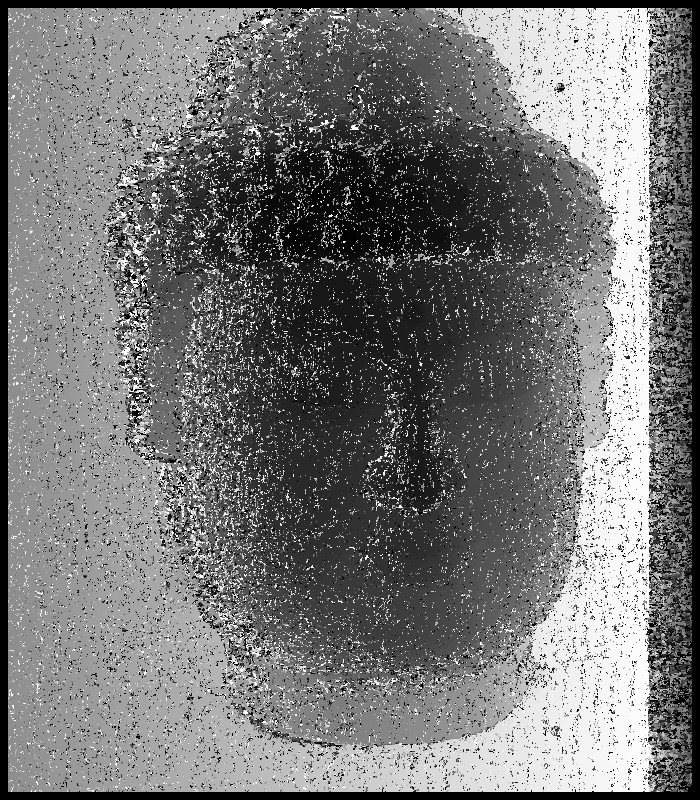
\includegraphics[height=60mm]{FIGS/Boudhas/Px1-Param0.jpg}
\hspace{10 mm}
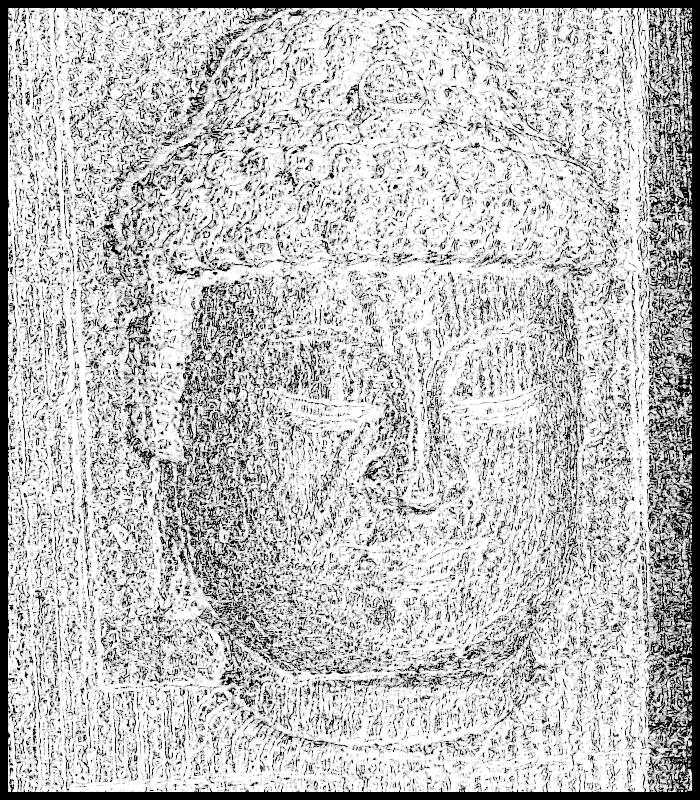
\includegraphics[height=60mm]{FIGS/Boudhas/CorrelParam0.jpg}
\caption{Disparity map an correlation image, dynamic has been adapted}
\label{FIG:DISP:COR:BASIC}
\end{figure}

%-------------------------------------------------------------------
%-------------------------------------------------------------------
%-------------------------------------------------------------------

\section{Examples Using MicMac, Algorithmic Aspect}


\subsection{Using Multi-resolution}

\label{BASIC:MULRES}

The file {\tt Param-1-Epi.xml} adds the multi-resolution aspect 
to the previous one. The modified or added parts from
{\tt Param-0-Epi.xml} are:


{\scriptsize
\begin{verbatim}
        ....
        <EtapeMEC>
               
              ...
             <Px1DilatAlti>  3    </Px1DilatAlti>
             <Px1DilatPlani> 4    </Px1DilatPlani>
             <!-- Unused here  but mandatory -->
             <Px1Regul>  0    </Px1Regul>
        </EtapeMEC>


        <EtapeMEC> <DeZoom >        8        </DeZoom> </EtapeMEC>
        <EtapeMEC> <DeZoom >        4        </DeZoom> </EtapeMEC>
        <EtapeMEC> <DeZoom >        2        </DeZoom> </EtapeMEC>
        <EtapeMEC> <DeZoom >        1        </DeZoom> </EtapeMEC>
        <EtapeMEC>
                 <DeZoom >        1        </DeZoom>
                 <Px1Pas>        0.5  </Px1Pas>
        </EtapeMEC>
        ...

\end{verbatim}
}

The principle of the multi-scale matching is that real homologous points are similar
at every scale, while "false" homologous points that may appear, by hazard, at a certain
scale will not be similar at other scales. To implement this idea, MicMac computes
a pyramid of images at scale $1,2,4,8 \dots$, and tries to compute a matching that
selects points who are similar in all the specified scales. The directory
{\tt Pyram-Epi/} specified by the tag {\tt TmpPyr} contains the file at different
resolutions with a quite obvious name ({\tt Epi-Left.tifDeZoom8.tif}  for
image {\tt Epi-Left.tif} reduced of a factor $8$). As they are floating images,
you may have a problem to visualize them with most of the viewers. Figure~\ref{FIG:IM:MULRES}
presents some levels of the pyramid.


\begin{figure}
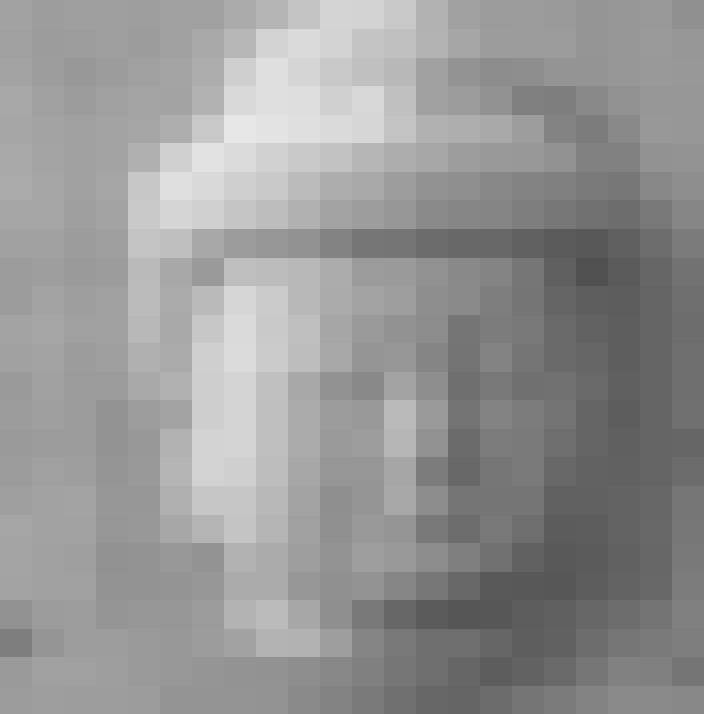
\includegraphics[height=40mm]{FIGS/Boudhas/Pyr32.jpg}
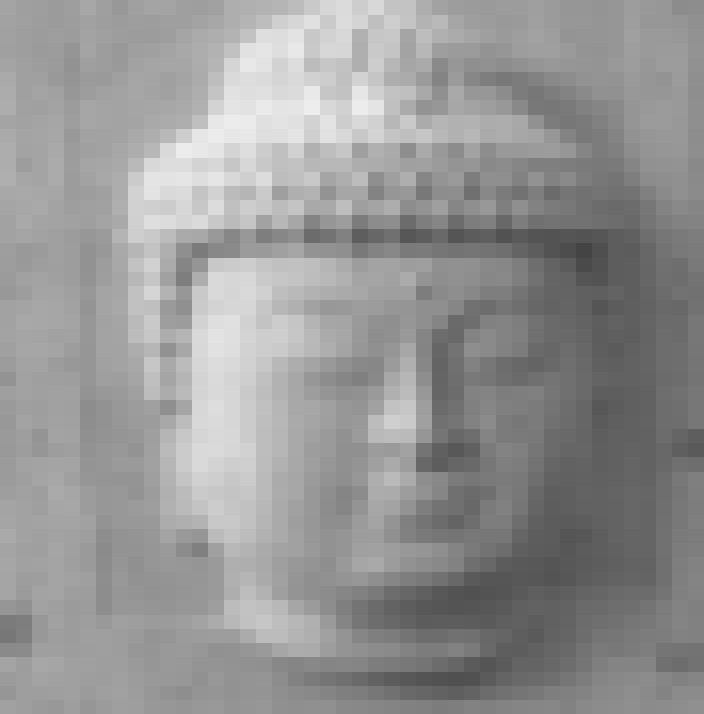
\includegraphics[height=40mm]{FIGS/Boudhas/Pyr16.jpg}
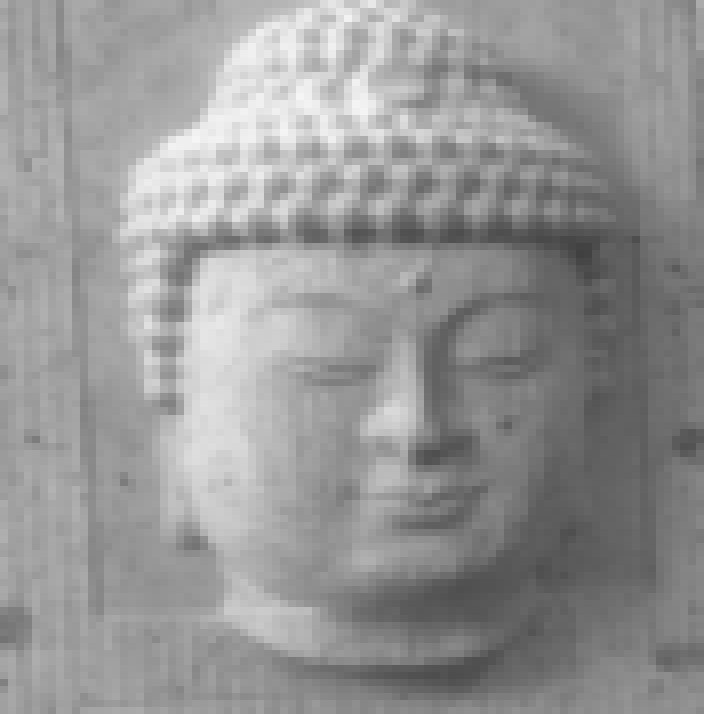
\includegraphics[height=40mm]{FIGS/Boudhas/Pyr8.jpg}
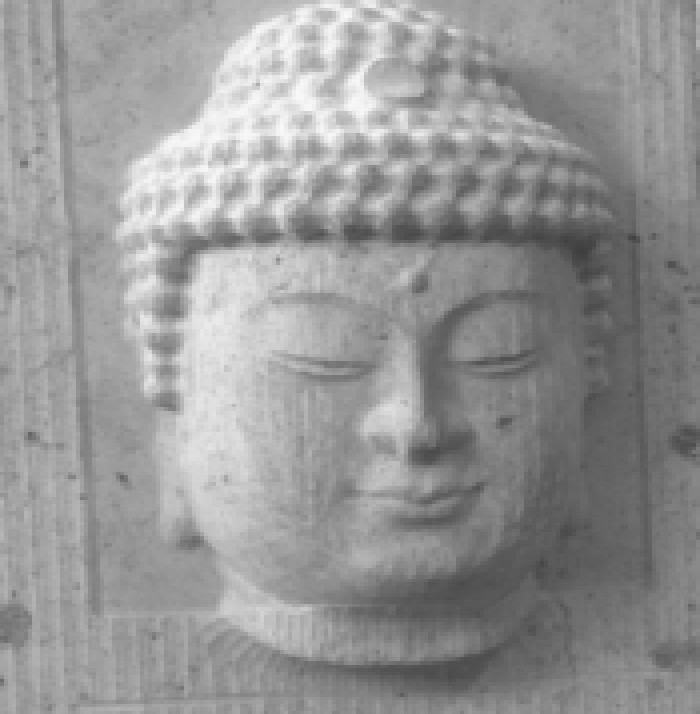
\includegraphics[height=40mm]{FIGS/Boudhas/Pyr4.jpg}
\caption{Some levels of the Buddha pyramid (the low resolution has been scaled so
     that all images have the same size in document)}
\label{FIG:IM:MULRES}
\end{figure}

MicMac does not process all the resolutions at the same time; in fact, it begins
with the lower resolution (here $8$). This lower resolution is treated "normally"
(i.e. without multi-scaling). Then iteratively, the resolution $2^n$ is computed,
using the solution $2^{n+1}$: MicMac forces the solution $2^n$ to be close
to the previous $S(2^{n+1})$. How much $S(2^n)$ must be close to  $S(2^{n+1})$ is
controlled by the paramaters {\tt Px1DilatAlti} and {\tt Px1DilatPlani}.
How these parameters are precisely used is described in~\ref{Appr:Multi:Resol}.

At each step, the computed disparity maps are saved and they  can be seen  in
directory {\tt MEC-1-EPI}:

\begin{itemize}
   \item {\tt Px1\_000\_DeZoom8\_LeChantier.tif} is a special case, it is
        full of zero, and computed to initiate the iterative process;


   \item the first computed disparity is {\tt Px1\_Num1\_DeZoom8\_LeChantier.tif} where
          the {\tt Num1} means first computed and {\tt DeZoom8}; the DeZoom is
          not sufficient as identifier as there are currently different phases at the
           same resolution; here, for example, Num4 and Num5; 

   \item this naming is a bit tricky, like almost all automatically generated names.

\end{itemize}

Figure~\ref{FIG:DISP:MUL:RES} shows levels of the pyramid of computed disparity maps.

\begin{figure}
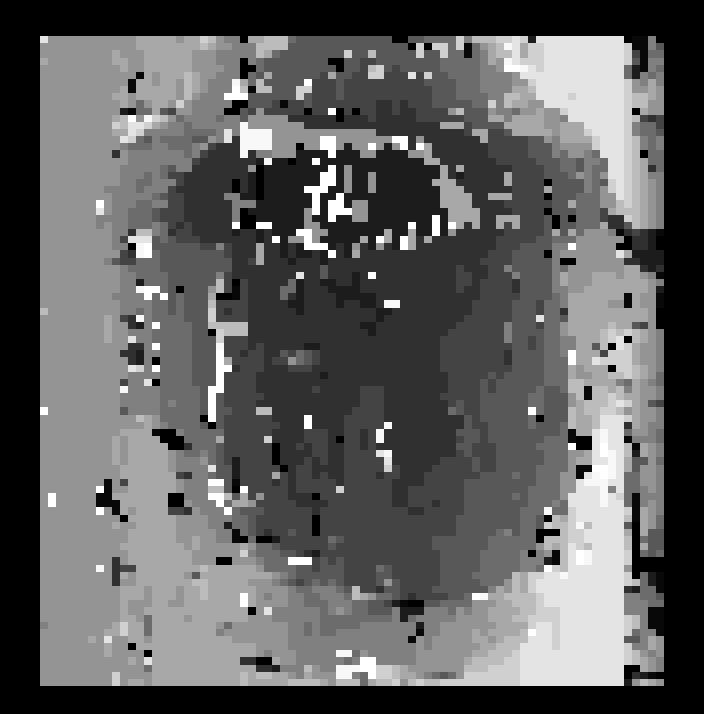
\includegraphics[height=40mm]{FIGS/Boudhas/Px1_MR_Num1.jpg}
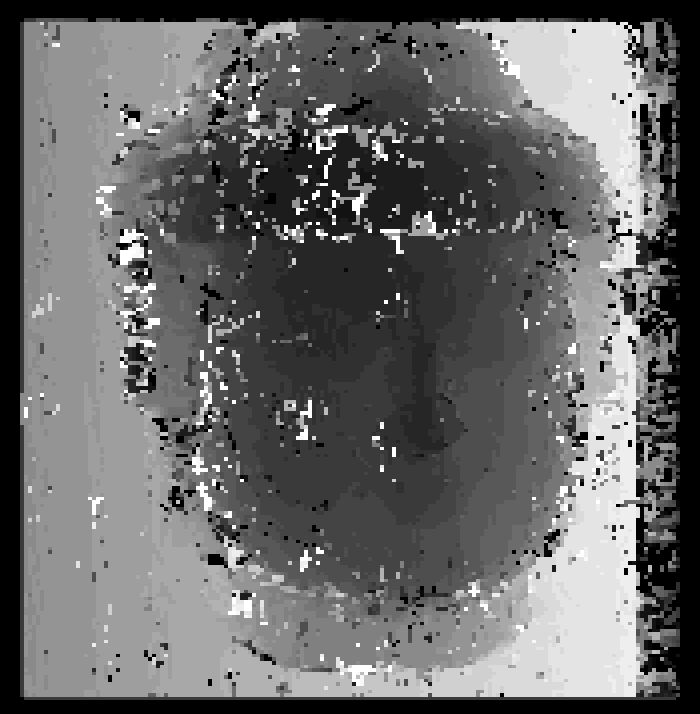
\includegraphics[height=40mm]{FIGS/Boudhas/Px1_MR_Num2.jpg}
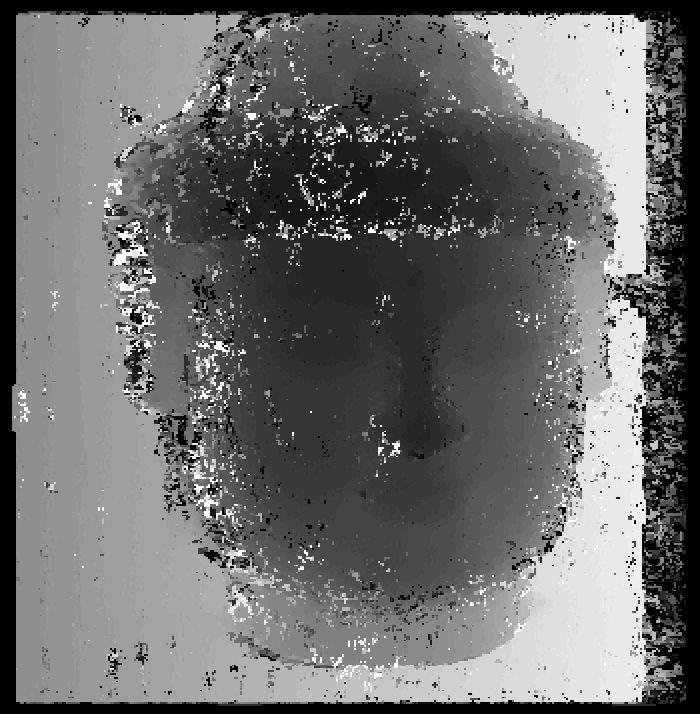
\includegraphics[height=40mm]{FIGS/Boudhas/Px1_MR_Num3.jpg}
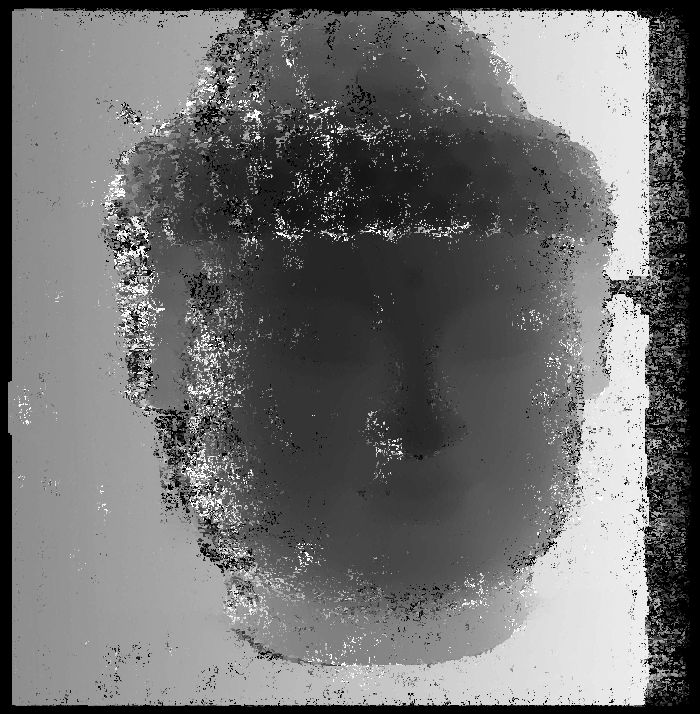
\includegraphics[height=40mm]{FIGS/Boudhas/Px1_MR_Num4.jpg}
\caption{The disparity maps computed at different resolutions}
\label{FIG:DISP:MUL:RES}
\end{figure}



If you compare the left image of figure~\ref{FIG:DISP:COR:BASIC} with the
right image of figure~\ref{FIG:DISP:MUL:RES}, you can observe that with the 
multi-scale approach the level of noise decreases.  Moreover, as this
multi-scaling is implemented via multi-resolution, the computation time
generally decreases very significantly.


With highly modern high quality camera and multi-stereoscopic acquisition,
it is possible to have a matching precision much better than the pixel.
To obtain  this sub-pixelar precision, a step parameter can be set with
the tag  {\tt Px1Pas}. Let $Step$ be the value of this parameter,
MicMac will compute the disparity:

     $d(x,y) = ArgMax_{d\in[-D,D]} Corr(x,y,x+d*Step,y,Sz)$;

Instead of :

     $d(x,y) = ArgMax_{d\in[-D,D]} Corr(x,y,x+d,y,Sz)$;

Of course we need to get values of images at non integer point, so
it requires an interpolation schema. In the previous example, the last phase 
was specified with a precision of half a pixel:


{\scriptsize
\begin{verbatim}
        <EtapeMEC>
                 <DeZoom >        1        </DeZoom>
                 <Px1Pas>        0.5  </Px1Pas>
        </EtapeMEC>
\end{verbatim}
}


The figure~\ref{FIG:DISP:PB:DISC} presents the effect
of this sub-pixellar matching.

\begin{figure}
\begin{center}
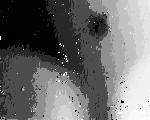
\includegraphics[height=60mm]{FIGS/Boudhas/Px1-Num4-PbDisc.jpg}
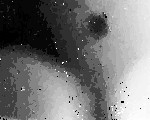
\includegraphics[height=60mm]{FIGS/Boudhas/Px1-Num5-PbDisc.jpg}
\caption{Zoom on a detail to illustrate the effect of the step parameter, left $step=1$ and right $step=0.5$}
\label{FIG:DISP:PB:DISC}
\end{center}
\end{figure}

\subsection{Using Regularization}

The file {\tt Param-2-Epi.xml} adds the regularization aspect
to the previous one. The modified or added  parts from
{\tt Param-0-Epi.xml} are:

{\scriptsize
\begin{verbatim}
         ....
             <AlgoRegul>    eAlgoCoxRoy    </AlgoRegul>
             <Px1Regul>  0.05    </Px1Regul>
             <ModeInterpolation> eInterpolMPD </ModeInterpolation>
         ....

       <EtapeMEC>
                 <AlgoRegul>    eAlgoDequant    </AlgoRegul>
                 <DeZoom >        1        </DeZoom>
                 <Px1Pas>         1  </Px1Pas>
        </EtapeMEC>
        ....

\end{verbatim}
}

The line {\tt ModeInterpolation> eInterpolMPD </ModeInterpolation>} shows
just how the interpolator, necessary for sub-pixel matching, is controled.


For the regularization, MicMac uses an energetic formalism, where a
functional, combining a regularity term and a image matching,
is globally minimized. Mathematical details can be found in
chapter~\ref{DUMG:Appr:Energ}. As several algorithms
are proposed, the tag  {\tt<AlgoRegul>} controls which
algorithm is to be chosen.  Here, the line
{\tt<AlgoRegul>    eAlgoCoxRoy    </AlgoRegul>}  correponds to
the Cox-Roy implementation of the Min-Cut/Max-Flow algorithm.

All theses algorithms have a parameter which allows to adjust 
the importance of regularity term relatively to the image term.
The tag {\tt Px1Regul} controls the value of this
parameter. Figure~\ref{FIG:DISP:REGUL} illustrates the results
of regularization.


\begin{figure}
\begin{center}
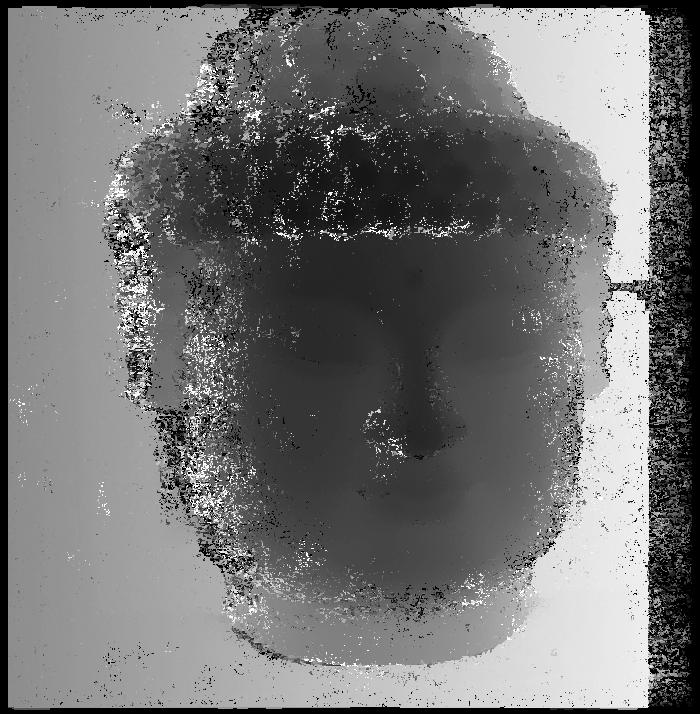
\includegraphics[height=55mm]{FIGS/Boudhas/Px1_MR_Num5.jpg}
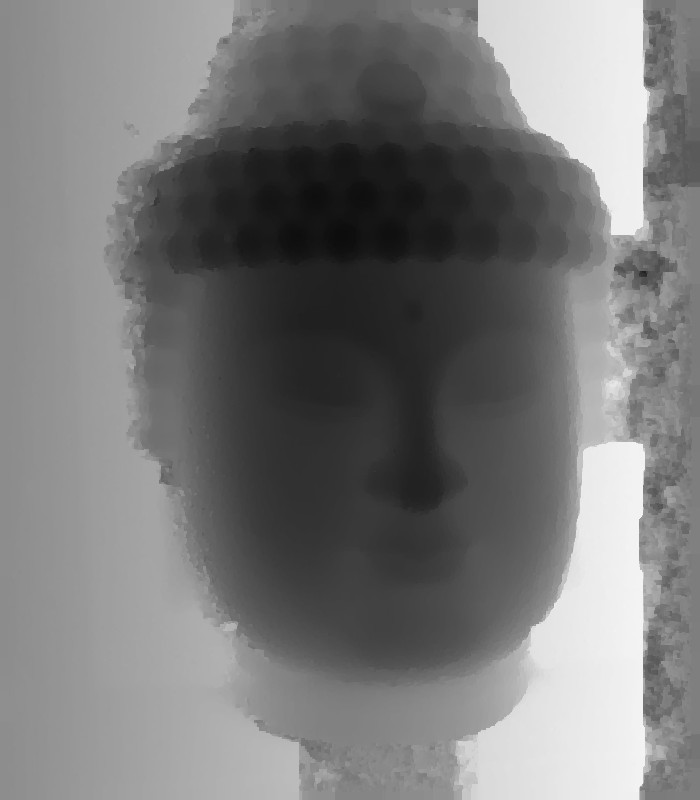
\includegraphics[height=55mm]{FIGS/Boudhas/Px1_REGUL_Num5.jpg}
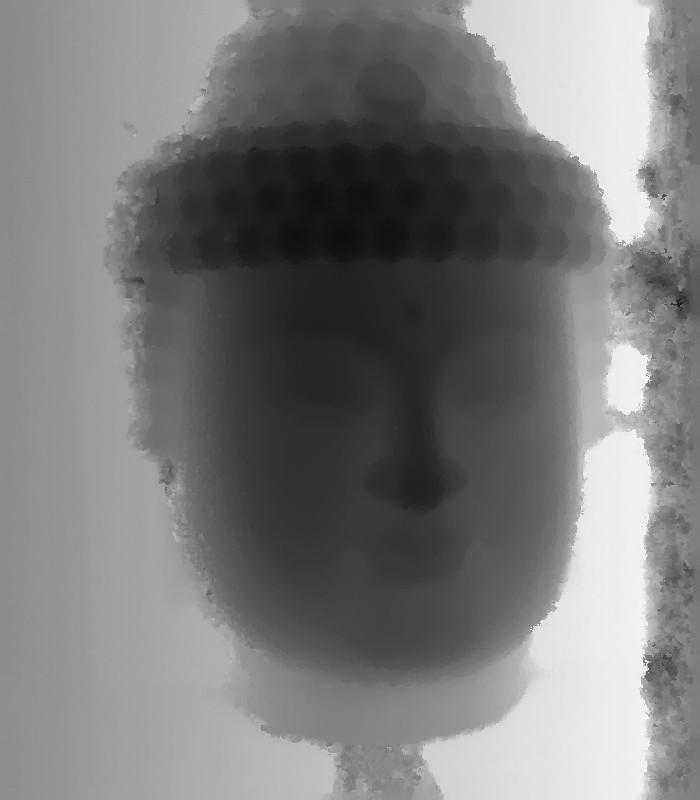
\includegraphics[height=55mm]{FIGS/Boudhas/PX1-Regul-ProgDyn.jpg}
\caption{Without regularization, with Graph Cut regularization, 
with 2D dynamic regularization}
\label{FIG:DISP:REGUL}
\end{center}
\end{figure}


In file {\tt Param-2-Epi.xml} the last and $6^{th}$ phase contains
the line {\tt <AlgoRegul>    eAlgoDequant    </AlgoRegul>}.
The matching algorithm used by MicMac makes a quantification
of the disparity (or depth, or height \dots, according to the geometry). 
This quantification creates jumps in the results that may be undesirable.
The dequantification algorithm, specified by {\tt  eAlgoDequant}, is
a post-processing phase that fixes 
the quantification artifacts.
This algorithm is described in~\ref{DUMG:DEQUANTIF}. The result is
a floating point map. MicMac imposes the step $1.0$ when using this algorithm
(as the notion of step is not pertinent for a floating point
result). Figure~\ref{FIG:DISP:REGUL} illustrates the effect of dequantification.




\begin{figure}
\begin{center}
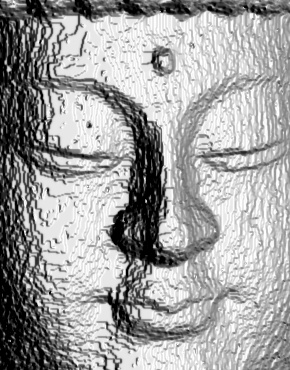
\includegraphics[height=60mm]{FIGS/Boudhas/ShadeQuant.jpg}
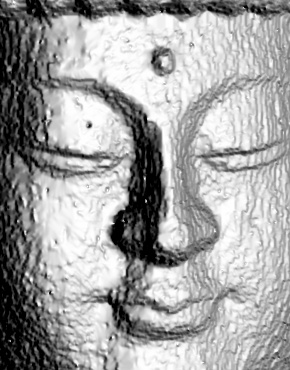
\includegraphics[height=60mm]{FIGS/Boudhas/ShadeDeQuant.jpg}
\caption{Without and with dequantification}
\label{FIG:DISP:REGUL}
\end{center}
\end{figure}


The file {\tt Param-3-Epi.xml} is similar to {\tt Param-2-Epi.xml}, the
main difference being the used regularization algorithm. It is specified 
{\tt eAlgo2PrgDyn} which is a $2D$ generalization of dynamic programming.
This algorithm does not produce the exact minimum of the energy function,
but a solution generally very close to the optimum. On the other hand,
it is generally faster and more flexible. It has more parameters;
the lines of {\tt Param-3-Epi.xml} corresponding to a basic
parametrization are:

{\scriptsize
\begin{verbatim}
         ....
            <ModulationProgDyn>
                 <EtapeProgDyn>
                      <ModeAgreg> ePrgDAgrSomme </ModeAgreg>
                      <NbDir>   7               </NbDir>
                  </EtapeProgDyn>
                  <Px1PenteMax>   3.0    </Px1PenteMax>
            </ModulationProgDyn>
        ....

\end{verbatim}
}

The \UNCLEAR{middle} %il y a seulement deux images dans fig 3.7
 and right images of figure~\ref{FIG:DISP:REGUL}  allow to compare the result
of max flow algorithm and 2D dynamic programming.

In {\tt Param-3-Epi.xml}, the line {\tt  <GenImagesCorrel > true </GenImagesCorrel> }
requires to generate the correlation coefficient image for every phase
(otherwise, it is generated only for the last phase). The file name  is
easy to understand, for example  {\tt Correl\_LeChantier\_Num\_3.tif}.


Another innovation of {\tt Param-3-Epi.xml} is {\tt  <ByProcess> 2 </ByProcess>} in
section {\tt Section\_WorkSpace}. With this option, MicMac will have the ability
to split the computation in two parallel processes. With my computer, I set
{\tt  <ByProcess>} at $2$, because I have only two processor, but if you have,
for example $4$ bi-processor, you can set it at $8$. Of course, it is your responsability
to set it to a reasonable value, knowing the characteristics of your computer
and other tasks that may be runinng at the same time.

%-------------------------------------------------------------------
%-------------------------------------------------------------------
%-------------------------------------------------------------------

\section{Examples using MicMac, Geometric Aspect}

To run the example coming in this section, you need to have executed the shell 
described in~\ref{SHEL:TEST:BOUDHA}
because it generates the required orientation files.

Figure~\ref{FIG:ALL:BOUDHA} presents a quick view of the $34$
images that will be used to illustrate full $3D$ modelization
with Apero and MicMac.

\begin{figure}
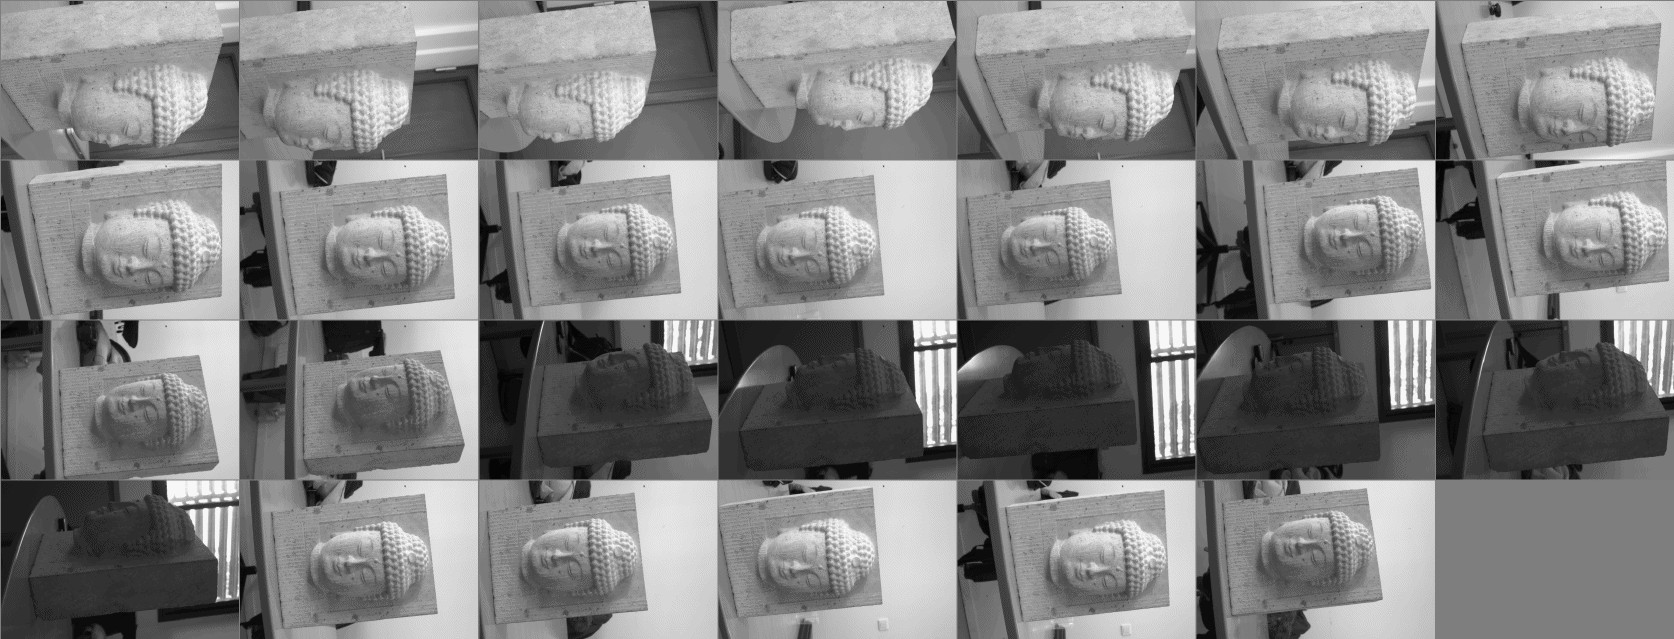
\includegraphics[width=150mm]{FIGS/Boudhas/Planche.jpg}
\caption{The $34$ images used in the following section}
\label{FIG:ALL:BOUDHA}
\end{figure}

       %  - - - - - - - - - - - - - - - - - - -

\subsection{Ground Geometry}

\label{Ground:Geom}

Epipolar geometry has the advantage of simplicity.  However, it lacks
of generality, it cannot be used for multi-stereoscopy and it imposes
unnecessary ressampling of the images. Moreover, generating proper epipolar
images requires some preliminary orientation of the image, so potentially
if you can do epipolar geometry, you will be able to do ground geometry. There
are almost no case where epipolar matching is preferable.

Mathematically, the object defining the orientation of an image $k$ is
a function  $\pi_k: \RR^3 \rightarrow \RR^2$; $\pi_k(x,y,z)=(i,j)$
where $(x,y,z)$ is a ground point and $i,j$ its projection in image
$k$.  The model understood by MicMac can be:


\begin{itemize}
   \item  stenope projection, which is adapted to all current cameras;
         the model is $\pi_k(x,y,z) = I (p_0 (R_k((x,y,z)-C_k)))$,
         where $I$ is the intrinsic parameters (focal, principal point and
         distorsion) and $p_0(x,y,z)=\frac{(x,y)}z$;
         the imported stenope model can be in different formats such as 
         XML coming from the Apero software and several formats used at IGN;

   \item  different generic model (Grid model of RPC, ratio of polynomial) 
          adapted to non physical modelization of push-broom images (satellites ...);

   \item the user can add its own model using a dynamic library (a bit tricky \dots).

\end{itemize}


In this example we will consider only stenope model stored in the format
generated by Apero. The matching in ground geometry consists in computing a
height map $Z=Z(x,y)$ so that:


\begin{itemize}
   \item   the windows centered on the $I_k(\pi_k(x,y,Z(x,y)))$  are similar;
   \item   $Z(x,y)$ satisfies some regularity function.
\end{itemize}

All the algorithmic points studied for epipolar disparity maps, are usable for 
ground geometry height map.

       %  - - - - - - - - - - - - - - - - - - -

\subsection{An Example in Ground Terrain, Parameter Analysis}


\label{FIRSTASSOC:LOC}
The file {\tt Param-4-Ter.xml} is our first example of matching in ground geometry.
It uses multi-stereoscopy matching with the five images of figure~\ref{FIVEBOUDHA}.
It contains several innovations:

{\scriptsize
\begin{verbatim}
   ....
<!--  M1 : Declare an association between an image and its orientation file-->
<DicoLoc>   
    <KeyedNamesAssociations>
        <Calcs>
            <Direct>
                <PatternTransform> (.*) </PatternTransform>
                <CalcName>  Ori-Test-5/Orientation-$1.xml  </CalcName>
             </Direct>
        </Calcs>
        <Key>   Loc-Key-Orient </Key>
    </KeyedNamesAssociations>
</DicoLoc>

<!--  M2 : Describe the ground zone where the matching is to be done -->
<Section_Terrain>    
      <IntervAltimetrie>
             <ZIncCalc>   3.0  </ZIncCalc>
      </IntervAltimetrie>
      <Planimetrie>
           <BoxTerrain> -2.13 -2.56 3.51 5.08 </BoxTerrain>
      </Planimetrie>

</Section_Terrain>

<!--  M3 : describe the set of images to match -->
<Section_PriseDeVue >   
     <GeomImages> eGeomImageOri </GeomImages>
     <Images >
          <ImPat> IMG_[0-9]{4}.tif </ImPat>
          <Filter>
              <Min>  IMG_5588.tif  </Min>
              <Max>  IMG_5592.tif </Max>
           </Filter>
     </Images>

     <NomsGeometrieImage>
         <FCND_Mode_GeomIm>
               <FCND_GeomCalc> Loc-Key-Orient  </FCND_GeomCalc>
         </FCND_Mode_GeomIm>
     </NomsGeometrieImage>
</Section_PriseDeVue>
   ...
<!--  M4 : Specify the output geometry -->
<Section_Results >
    <GeomMNT> eGeomMNTEuclid  </GeomMNT>
</Section_Results>

\end{verbatim}
}

\begin{figure}
\begin{center}
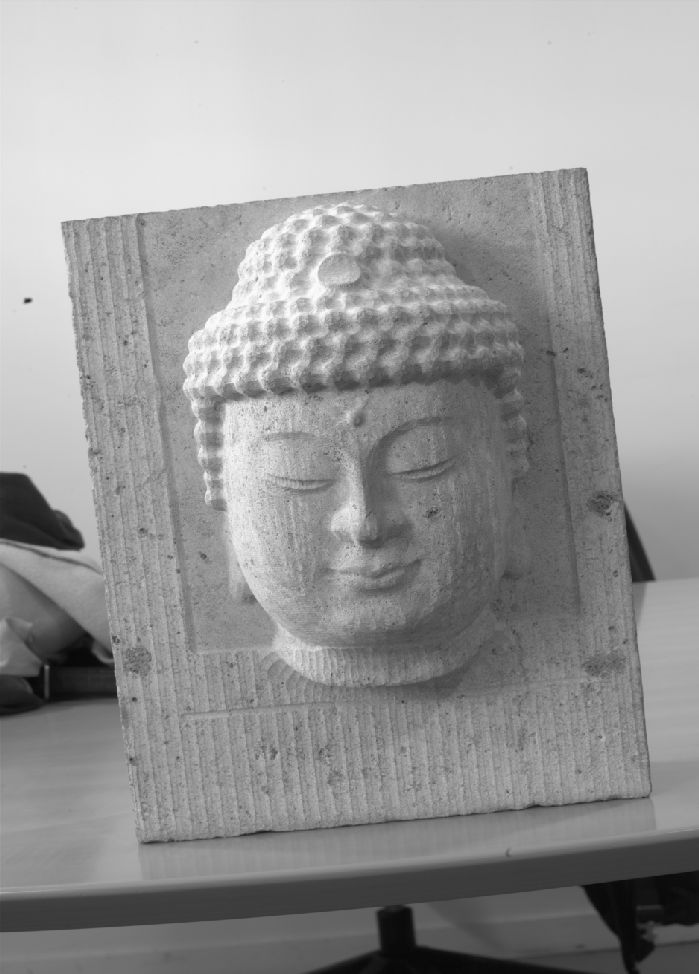
\includegraphics[height=55mm]{FIGS/Boudhas/IMG_5588.jpg}
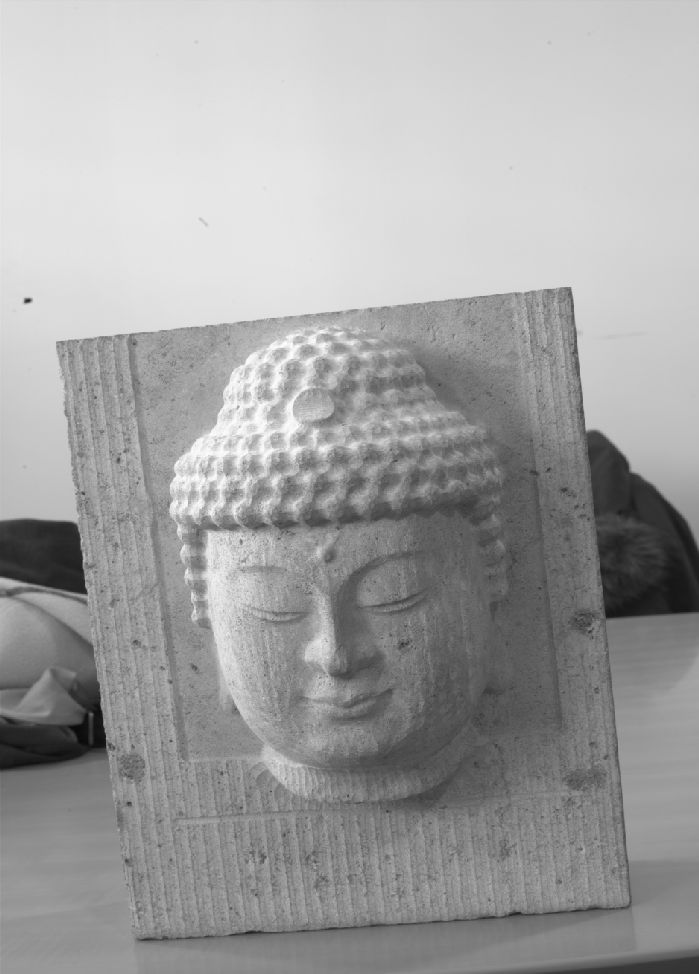
\includegraphics[height=55mm]{FIGS/Boudhas/IMG_5589.jpg}
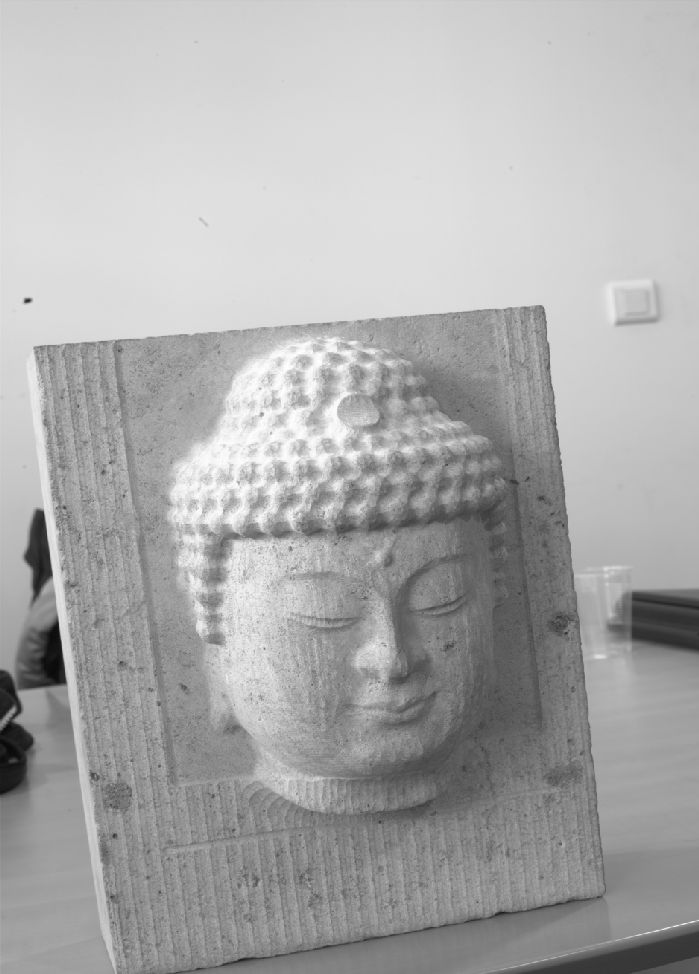
\includegraphics[height=55mm]{FIGS/Boudhas/IMG_5590.jpg}
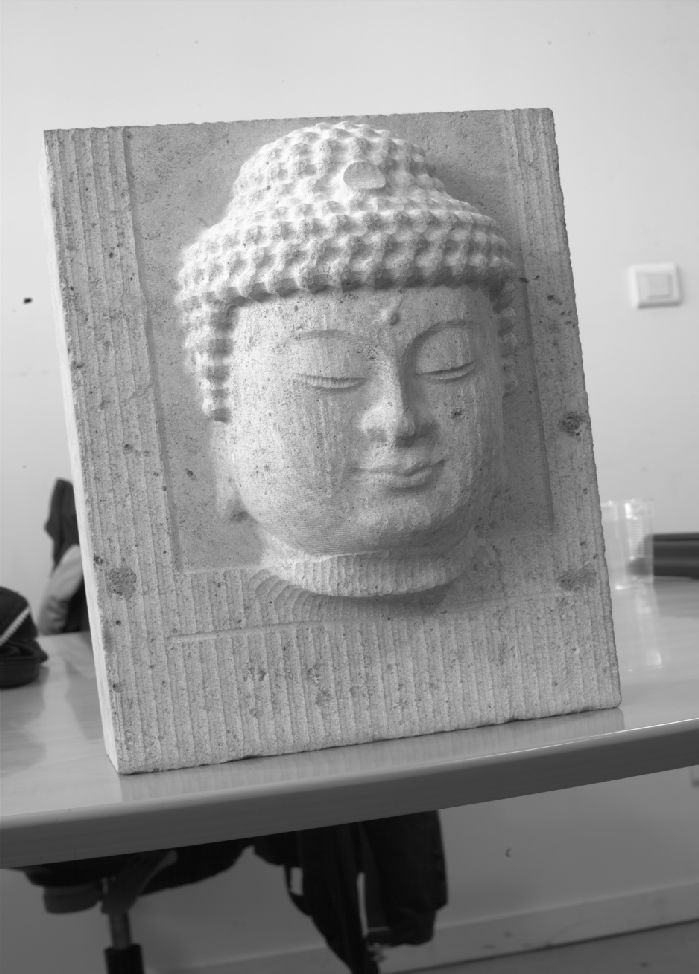
\includegraphics[height=55mm]{FIGS/Boudhas/IMG_5591.jpg}
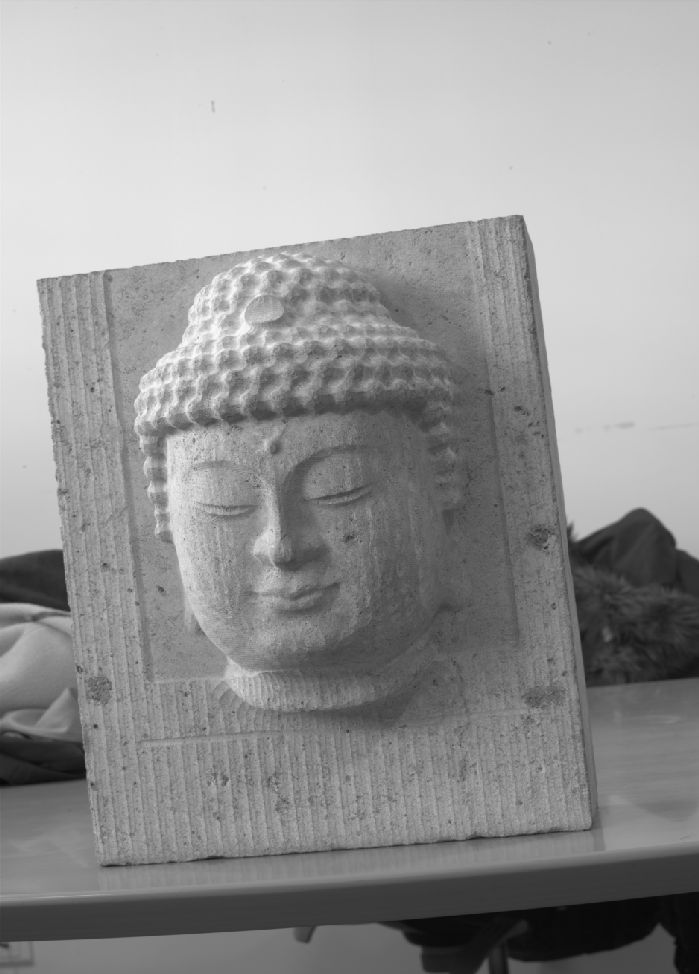
\includegraphics[height=55mm]{FIGS/Boudhas/IMG_5592.jpg}
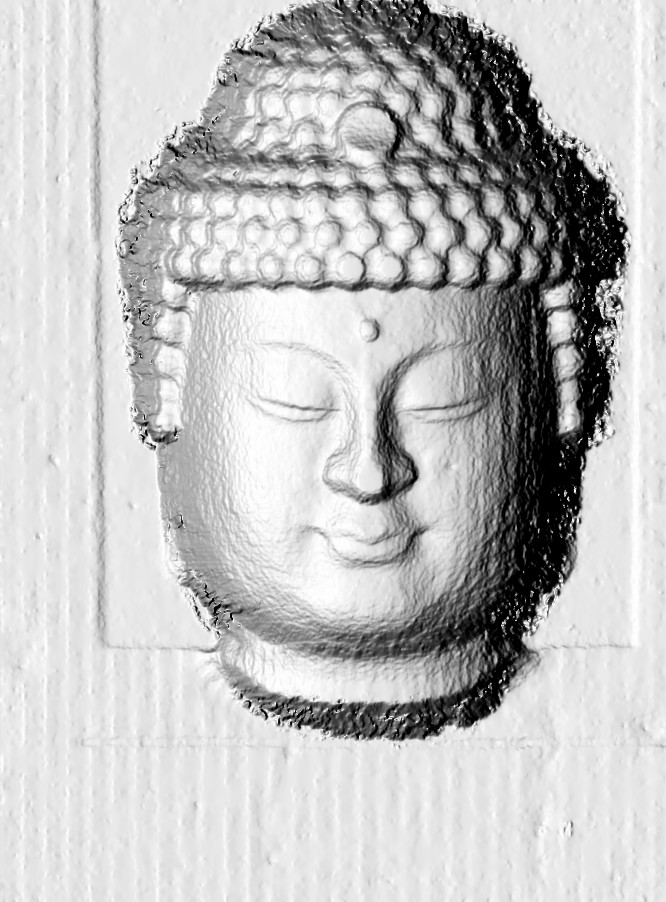
\includegraphics[height=55mm]{FIGS/Boudhas/Terrain-Shade.jpg}
\caption{The five images used for ground geometry matching, and a shading of the DTM}
\label{FIVEBOUDHA}
\end{center}
\end{figure}

The first new tag, {\tt <DicoLoc>}, is an example of how the user can
describe the association between the name of an image and the name
of its orientation file:

\begin{itemize}
   \item  the pair of tags {\tt  <PatternTransform>} and {\tt <CalcName>} declares an
          association rule; this rule means, for example, that the orientation of {\tt IMG\_5580.tif}
          is located in the file \newline
          {\tt Ori-Test-5/Orientation-IMG\_5580.xml};

    \item this rule means, for example,  that the orientation of  {\tt IMG\_5580.tif}
          is located in the file \newline {\tt Ori-Test-5/Orientation-IMG\_5580.tif.xml};
    \item take a quick look to a file {\tt Ori-Test-5/Orientation-IMG\_.*.xml} and
         the file  {\tt Ori-Test-5/AutoCalib.xml}; if you have some idea of what
         a stenope projection is, you should understand the main principle of the used format;
         the section~\ref{FORM:CALIB} gives a formal description of the format;

    \item  to this rule it is given an identifier, here {\tt Loc-Key-Orient}; when it is necessary 
    		to refer to this association rule, this key will be used;

    \item  generally, the mechanism allowing the declaration directly in the MicMac
           parameter is to be avoided; it is preferable to use predefined rules or to declare
           them in the special file \newline {\tt MicMac-LocalChantierDescripteur.xml} to
           facilitate convention sharing and maintenance
           (I did it here, this time, for the simplicity of reading);
\end{itemize}

Here, orientations have been computed with Apero in a purely relative way. The orientations
are defined up to a global rotation, translation and scaling. An option of Apero has been
used to orientate the set of images so that the background plane is globally horizontal.

The second new tag, {\tt <Section\_Terrain>}, allows the user to enter the
information relative to the ground. The used options are :

\begin{itemize}
   \item  {\tt <ZIncCalc>} \UNCLEAR{specifies the amplitude of the incertitude interval that is to be explored;
          the central value is not specified here because the orientation file contains sufficient
          information to evaluate};

   \item  {\tt <BoxTerrain>}  specifies the ground surface on wich the matching is to be done;
          if  this  parameter is omitted, MicMac will automatically compute a surface which corresponds
          to the ground points seen at least in
          two images (at the average height); however, this would not be suitable
          here because it would include the background which we do not want to modelize.

\end{itemize}


The third innovation, {\tt <Section\_PriseDeVue>}, describes, in a manner adapted to ground geometry,
the way the scene was shooted :


\begin{itemize}
   \item the tag {\tt eGeomImageOri} specifies that the images were acquired by stenope
         camera \footnote{Of course, using only XML-type files, this information is already
         existing in orientation files, but it is necessary for historical reasons};

    \item the tag {\tt ImPat} specifies the images which are to be used for matching; we want
          to do multi-stereo matching but not necessarly with all the images existing in the
          directory, so we need a way to specify the set of images; there are many ways to
          do it, the most current ones are:

\begin{itemize}
        \item like this example, by giving a general pattern and {\tt Filter} including the name
              of the image, the selected image will verify $Min \leq Name \leq Max$ according
              to lexicographical order;
        \item by specifying a pattern using the power of regular expressions, here it would be
              equivalent to say {\tt <ImPat> IMG\_((558[8-9])|(559[0-2])).tif </ImPat>};
        \item as an arbirtrary number of tags {\tt ImPat} can exist, it will be alright to
             have {\tt <ImPat> IMG\_5588.tif </ImPat> <ImPat> IMG\_5589.tif </ImPat> \dots}

\end{itemize}

    \item the section in the tree {\tt NomsGeometrieImage} specifies that the key {\tt Loc-Key-Orient}
          declared above is to be used for getting the orientation name associated to an image.

\end{itemize}



       %  - - - - - - - - - - - - - - - - - - -

\subsection{An Example in Ground Terrain, Result Analysis}

\label{Ex:GrTer:RA}

Finally, the value {\tt eGeomMNTEuclid} of {\tt GeomMNT} specifies that the output 
geometry  is  \UNCLEAR{equal} to the input geometry.  This means that the resulting image
is, up to translation and scaling, directly understood as a grid $Z=f(x,y)$.
In fact, the value of the orientation file specifies the input geometry, but
there are many cases where we do
not want the computation to be done in this geometry \footnote{sometimes for exploitation
purpose, sometimes for quality of matching}. The most current case offered by MicMac
is the "ground-image" geometry presented in the example in~\ref{EX:TER:IM:GEOM}. There
is also the possibility of working in cylindrical geometry \footnote{it would be
interesting to offer the possibility to work directly in different geodetic-cartographic
systems, planed it for a long time, but still to be done}.

Here we work in "Euclidean" geometry, so the result is a grid $Z=f(x,y)$.
The bottom right image of figure~\ref{FIVEBOUDHA} shows, in shading mode,
the result obtained with this geometry. If we want to use this result
as a measurement tool, we will need more than an image; as it is a grid, we need some
information (meta-data)  to interpret it like a 3D model which we will
be able to import in another application (GIS, CAD \dots).

Take a look at directory {\tt MEC-4-Ter}. You will see that, to each
image file {\tt Z\_NumXXX\_DeZoomYYY\_LeChantier.tif} is associated a file
{\tt Z\_NumXXX\_DeZoomYYY\_LeChantier.xml}. For example, here is
{\tt Z\_Num3\_DeZoom2\_LeChantier.xml}:

{\scriptsize
\begin{verbatim}
<FileOriMnt>
      <NameFileMnt>/home/mpd/micmac_data/ExempleDoc/Boudha/MEC-4-Ter/Z_Num3_DeZoom2_LeChantier.tif</NameFileMnt>
      <NameFileMasque>/home/mpd/micmac_data/ExempleDoc/Boudha/MEC-4-Ter/Masq_LeChantier_DeZoom2.tif</NameFileMasque>
      <NombrePixels>333 451</NombrePixels>
      <OriginePlani>-2.12999999999999989 5.08000000000000007</OriginePlani>
      <ResolutionPlani>0.0169328251622493653 -0.0169328251622493653</ResolutionPlani>
      <OrigineAlti>0.380598155186812559</OrigineAlti>
      <ResolutionAlti>0.00846641258112469999</ResolutionAlti>
      <Geometrie>eGeomMNTEuclid</Geometrie>
</FileOriMnt>

\end{verbatim}
}

The important tags are {\tt <Origine..>} and {\tt <Resolution..>}. Let:

\begin{itemize}
   \item  $OriginePlani=X_0,Y_0$  ; 
   \item  $OrigineAlti=Z_0$       ;

   \item  $ResolutionPlani=\Delta_x,\Delta_y$       ;
   \item  $ResolutionAlti=\Delta_z$       ;
\end{itemize}

Then each point $I,J,K=K(I,J)$ of the grid defines an $x,y,z$ point by the basic formula:


\begin{equation}
   \begin{pmatrix}  x \\ y \\ z \end{pmatrix}
   = \begin{pmatrix}  X_0 + I * \Delta_x \\ Y_0 + J * \Delta_y \\ Z_0 + K * \Delta_z \end{pmatrix}
\end{equation}

Notice that in the parameter file there is no specification of planimetric resolution. 
In this case, we have to let MicMac make the choice; it has selected a ground resolution 
equal to the average resolution of the image, this is possible because the orientation
file generated by Apero contains the necessary information (like average height).
For the altimetric resolution, it is implicitly specified by the parameters
{\tt ZPas}: the altimetric resolution is equal to the  planimetric resolution
multiplied by {\tt ZPas}; this convention has the advantage that, for this point, the parameter
files are adaptable to a wide family of configurations.

       %  - - - - - - - - - - - - - - - - - - -

\subsection{An Example in "Ground-image" Geometry}

\label{EX:TER:IM:GEOM}

Having the output geometry \UNCLEAR{equal} to the input geometry is perfectly fine for the
modelization of quasi-planar objects: modelization of the earth surface seen for aerial
point of view, modelization of bas-reliefs\dots However it is not suited for the
modelization of fully 3-dimensional objects.  For this kind of modelization, MicMac
proposes the "image-ground" geometry in which the user can easily select a geometry
adapted to each point of view. There are several \UNCLEAR{variants} of this geometry; 
in all image-ground geometry, there is a master image $I_m$ and the $x,y$
of this geometry represents simply the pixel $I,J$ of $I_m$.
We describe here the $1D$-depth-of-field ($1D$dof)  which is optimized for well calibrated stenope camera.

The input geometry defines the correspondence between a point $x,y,z$ of
the Euclidean space and its projection in each image. To define the output
geometry we must define the correspondence beetween a point $A,B,C$ of
the \UNCLEAR{result} space and its homologous in Euclidean space $x,y,z$, in $1D$dof:

\begin{itemize}
   \item  $A,B$ represents a pixel of the master image $I_m$;
   \item  $C$ represents the inverse of the depth of field ;
   \item so $x,y,z$ is the point located on the ray emerging from $A,B$ and
         located at depth\footnote{depth(P)=distance between the optical center and the projection of P on the optical axis} $\frac1C$;
   \item the advantages of this geometry are:
\begin{itemize}
   \item like all the other ground-image geometries, the disparity map is directly superposable to 
          the first image;
   \item for a given ray, a regular sampling of  $\frac1C$ corresponds, as much as possible, to a regular sampling
         of the projection in all images; if $C$ was regularly sampled, with scenes having a very high depth
         of field, there would be no good choice for the quantization step;
    \item so this geometry has the advantage of the epipolar one, without the drawbacks.
\end{itemize}
\end{itemize}



\begin{figure}
\begin{center}
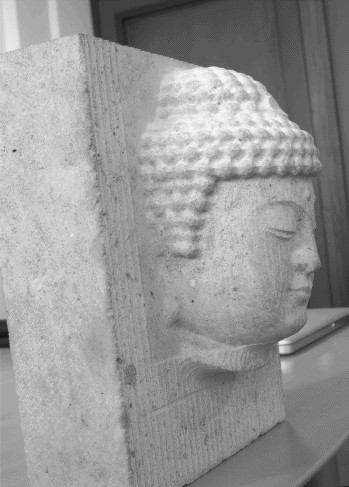
\includegraphics[height=55mm]{FIGS/Boudhas/IMG_5564.jpg}
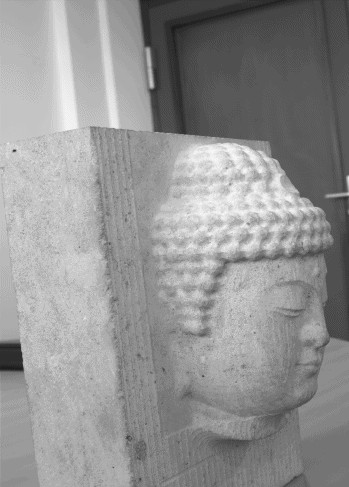
\includegraphics[height=55mm]{FIGS/Boudhas/IMG_5565.jpg}
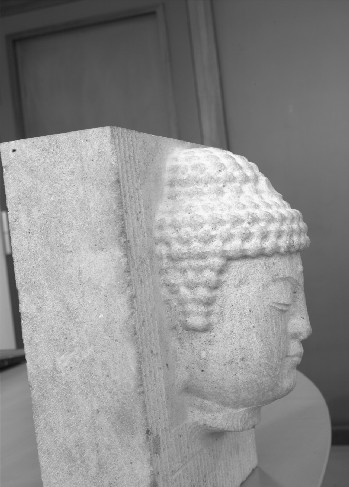
\includegraphics[height=55mm]{FIGS/Boudhas/IMG_5566.jpg}
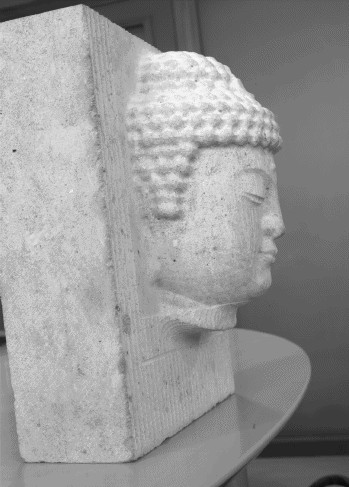
\includegraphics[height=55mm]{FIGS/Boudhas/IMG_5567.jpg}
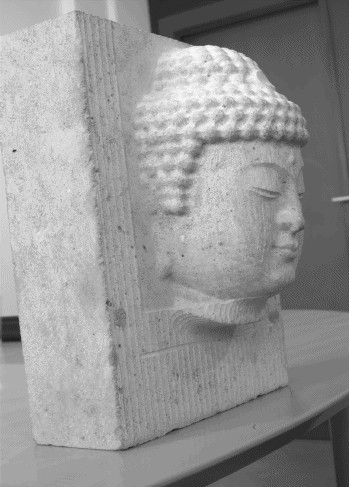
\includegraphics[height=55mm]{FIGS/Boudhas/IMG_5568.jpg}

\includegraphics[height=55mm]{FIGS/Boudhas/IMG_5564_Masq.jpg}
\caption{Input to matching for left face of Buddha: 5 image and a mask}
\label{BOUDHA:GRIM:INPUT}
\end{center}
\end{figure}

Now we want to make a $3D$ model of the left face of the Buddha, using
the $5$ images of figure~\ref{BOUDHA:GRIM:INPUT}. The file {\tt Param-5-Ter.xml}
gives an example of such paramatring, there are important differences with the previous file.

{\scriptsize
\begin{verbatim}
<Section_Results >
    <GeomMNT> eGeomMNTFaisceauIm1PrCh_Px1D  </GeomMNT>
</Section_Results>
\end{verbatim}
}

One difference, at the end of the file, just specify the kind of geometry:
the name is a bit strange\dots However {\tt FaisceauIm1} means \UNCLEAR{bundle} of image 1;
{\tt PrCh} is a short for "Profondeur de champs" (depth of field) and {\tt Px1D}
means $1D$ disparity\footnote{by opposition with variants allowing $2D$ match for
compensation of unprecise calibration}.


{\scriptsize
\begin{verbatim}
<Section_MEC >
      <ChantierFullImage1>  true </ChantierFullImage1>
....
<Section_MEC >
\end{verbatim}
}

The second difference means that we
want the computed depth image to be exactly superposable to the master image.
If we do not precise this point, MicMac may clip the space to a box containing
only the reachable pixels; so it is important.


{\scriptsize
\begin{verbatim}
<Section_PriseDeVue >
     <GeomImages> eGeomImageOri </GeomImages>
     <Images >
          <Im1> IMG_5564.tif </Im1>
          <ImPat> IMG_[0-9]{4}.tif </ImPat>
          <Filter>
              <Min>  IMG_5564.tif  </Min>
              <Max>  IMG_5568.tif </Max>
           </Filter>
     </Images>

     <NomsGeometrieImage>
         <FCND_Mode_GeomIm>
               <FCND_GeomCalc>  NKS-Assoc-Im2Orient@-Test-5  </FCND_GeomCalc>
         </FCND_Mode_GeomIm>
     </NomsGeometrieImage>
</Section_PriseDeVue>
....
\end{verbatim}
}

\label{SECASSOC:PRED}
The {\tt Section\_PriseDeVue} has two differences:

\begin{itemize}
   \item  to specify the image set we have two different tags {\tt Im1} and {\tt ImPat};
          in this geometry, as there is a master image that plays a special role, we need
          a way to indicate which is the master, this is the role of tag {\tt Im1};

   \item  we have no section {\tt DicoLoc} defining a rule for computing association, 
          instead, we have used {\tt NKS-Assoc-Im2Orient@-Test-5}, this is what is
          called a predefined parametrized key : 

\begin{itemize}
    \item  it is predefined, because the definition of the key is made in the file
           \newline {\tt include/XML\_GEN/DefautChantierDescripteur.xml} which contains a lot
           of predefined rules that are automatically loaded in all the tools;

    \item  it is parametrized, because here {\tt NKS-Assoc-Im2Orient} is the name of
           a parameterizable key and {\tt -Test-5} is the value of the parameter;
           in the definition of {\tt NKS-Assoc-Im2Orient} in \newline {\tt XML\_GEN/DefautChantierDescripteur.xml}
           you will find strings like {\tt Ori\#1/Orientation-\$1.xml}, each time {\tt \#1} is
           encountered it will be replaced by {\tt -Test-5};

     \item so {\tt NKS-Assoc-Im2Orient@-Test-5} is strictly equivalent to the definition that has been
           given in {\tt Loc-Key-Orient} in file {\tt Param-4-Ter.xml};

     \item it is hoped that the parametrized rule will be sufficient to cover $95\%$ of needs;
\end{itemize}
\end{itemize}


{\scriptsize
\begin{verbatim}
...
<Section_Terrain>
      <IntervAltimetrie>
             <!-- Mandatory but unused -->
             <ZIncCalc>   0.0  </ZIncCalc>
      </IntervAltimetrie>
      <IntervSpecialZInv >
             <MulZMin >  0.3</MulZMin>
             <MulZMax > 5 </MulZMax>
      </IntervSpecialZInv>
     <Planimetrie>
         <MasqueTerrain>
             <MT_Image> IMG_5564_Masq.tif </MT_Image>
             <MT_Xml> IMG_5564_Masq.xml </MT_Xml>
         </MasqueTerrain>
     </Planimetrie>
</Section_Terrain>
\end{verbatim}
}

The {\tt Section\_Terrain} has several differences:


\begin{itemize}
   \item  the value of {\tt ZIncCalc}, specifying an interval of $Z$, is set
          to $0$ , it will not be used because of the following tags {\tt IntervSpecialZInv};

   \item  the tag {\tt IntervSpecialZInv} specifies that the depth of field interval to
          explore is $[0.3*D_0, 5*D_0]$ where $D_0$ is the average depth (MicMac knows it
          from the information contained in the orientation files);

     \item the tag {\tt MT\_Image} contains information for a mask of the terrain points 
     		that are to be matched, the terrain points \UNCLEAR{refer} to the output geometry,
           here the pixels of the image {\tt IMG\_5564.tif}; figure~\ref{BOUDHA:GRIM:INPUT}
           contains an image of the mask used here; it has been created with the
           tool {\tt bin/SaisieMasq};

     \item the tag {\tt MT\_Xml} contains the name of the meta data file that georeferences
           the image file {\tt IMG\_5564\_Masq.tif}; this tag is important because
           when working on georeferenced data it may be necessary to use a mask,
           created on a GIS, at a step and resolution different from those chosen
           by MicMac; here, in the image geometry, it is not very informative (open it),
           however it is mandatory;
\end{itemize}




The left image of the figure~\ref{BOUDHA:CLOUD:INPUT} presents, in shading,
the result of the depth-map you will obtain. Often,  for $3D$ modelization,
what is needed is not a depth-map but a $3D$ point cloud. Due to the chosen geometry, 
several pieces of information are necessary to generate $3D$ points from
depth map:


\begin{itemize}
  \item  calibration of the camera (internal and external) to compute, for 
         each pixel, its ray in Euclidean space;
  \item  origin and steps of depth quantification;
  \item  mask of image;
  \item   the depth map itself.
\end{itemize}



\begin{figure}
\begin{center}
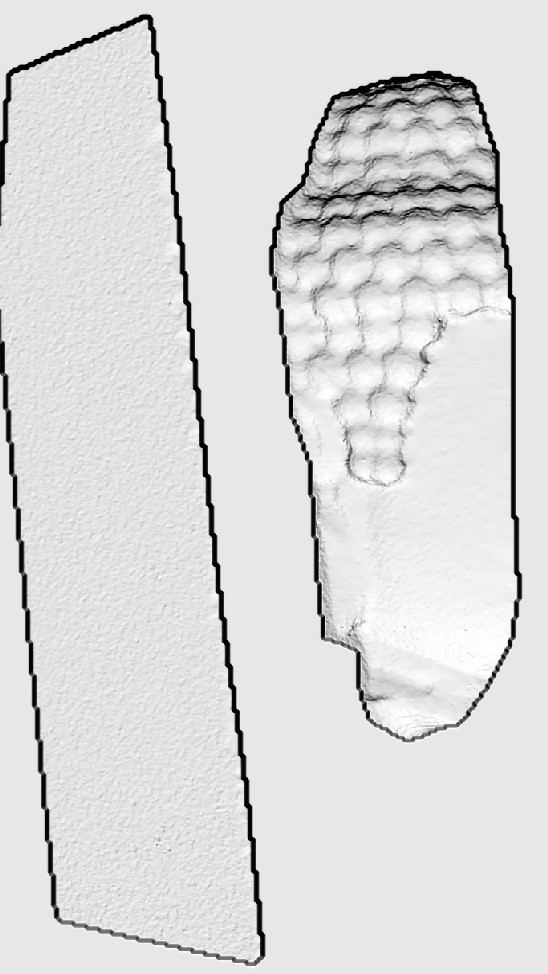
\includegraphics[height=55mm]{FIGS/Boudhas/FACE-Shade.jpg}
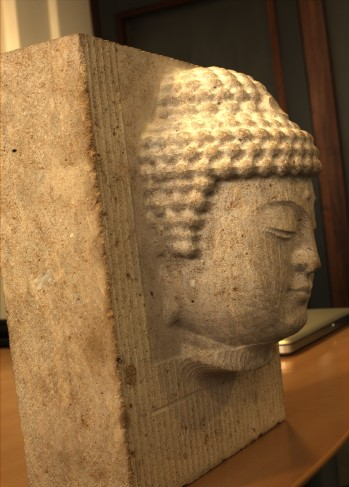
\includegraphics[height=55mm]{FIGS/Boudhas/IMG_5564-RGB.jpg}
\caption{Input to Cloud generation: depth map and RGB image}
\label{BOUDHA:CLOUD:INPUT}
\end{center}
\end{figure}


All these pieces of information exist in separated files and, once merged, they are sufficient 
to generate 3D points. For a greater convenience, files merging 
this information are generated. In directory {\tt MEC-5-Im/}
you will find the files {\tt NuageImProf\_LeChantier\_Etape\_X.xml}.
Take a look at these files, they contain all the information 
necessary to generate  the point clouds. There is only the conversion to do. 
The tool {\tt bin/Nuage2Ply} makes the conversion from
a file {\tt NuageImProf \dots} to a point cloud in {\tt ply} format.
For example, you can type:

\begin{verbatim}
bin/Nuage2Ply ../micmac_data/ExempleDoc/Boudha/MEC-5-Im/NuageImProf_LeChantier_Etape_5.xml \
   Attr=../micmac_data/ExempleDoc/Boudha/IMG_5564-RGB.tif 

\end{verbatim}

Here, the image {\tt IMG\_5564-RGB.tif} is a RGB image superposable to the master image
{\tt IMG\_5564.tif}. Figure~\ref{BOUDHA:CLOUD:INPUT} presents a view of this image. This 
command generates a file  {\tt NuageImProf\_LeChantier\_Etape\_5.ply} in the directory {\tt MEC-5-Im/}.
If you have the MeshLab tool, you will be able to visualize the cloud. Figure~\ref{BOUDHA:CLOUD:OUTPUT}
presents  some  viewpoints generated with MeshLab.
 


\begin{figure}
\begin{center}
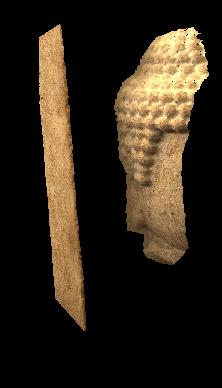
\includegraphics[height=55mm]{FIGS/Boudhas/PL-F1-A.jpg}
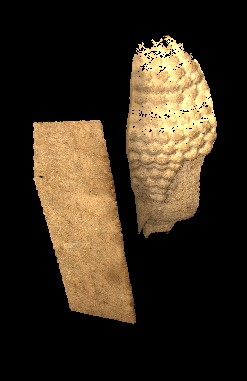
\includegraphics[height=55mm]{FIGS/Boudhas/PL-F1-B.jpg}
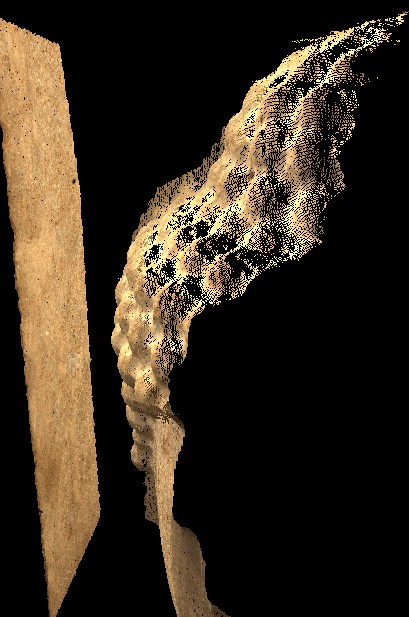
\includegraphics[height=55mm]{FIGS/Boudhas/PL-F1-C.jpg}
\caption{Some views of the generated point cloud}
\label{BOUDHA:CLOUD:OUTPUT}
\end{center}
\end{figure}


\subsection{Batching Several Computations}

Now we know  enough to build a complete $3D$ model of the
Buddha from the set of images presented on figure~\ref{FIG:ALL:BOUDHA}.
The Buddha is quite a simple object, so we can make the modelization with three
viewpoints. We just need to run $3$ times micmac with the following
parameters :


\begin{itemize}
   \item  for left viewpoint {\tt Im1=IMG\_5564.tif}, {\tt Min=IMG\_5564.tif} and {\tt Max⁼IMG\_5568.tif};
   \item  for central viewpoint {\tt Im1=IMG\_5588.tif}, {\tt Min=IMG\_5588.tif} and {\tt Max⁼IMG\_5592.tif};
   \item  for right viewpoint {\tt Im1=IMG\_5581.tif}, {\tt Min=IMG\_5581.tif} and {\tt Max⁼IMG\_5585.tif}.
\end{itemize}


The obvious way to do it would be to run with one set of parameters, wait for the computation to be over, 
modify the file of parameters, wait the \UNCLEAR{\dots} %il n'y a pas de suite pour wait
But imagine you have $30$ viewpoints to generate,
you do not want to spend hours in front of your computer, you want to specify once all your
matchings, start the computation and concentrate on other tasks while the computer works;
in other words, you need to batch the process.

If you are a computer programmer, you will be able to
easily build a program that generates and run MicMac with the good parameters; if
not, MicMac proposes a simple mechanism to do it. It is used
in the file {\tt Param-6-Ter.xml}.

First, the header is quite new :

{\scriptsize
\begin{verbatim}
<ParamMICMAC

     Subst="@$#1"
     NameDecl="@$#1"

     NumC="@5564"
     NumMin="@5564"
     NumMax="@5568"
>
\end{verbatim}
}

The syntax is a bit strange, and dangerous, so you will have to follow it
very carefully:

\begin{itemize}
   \item  {\tt Subst="@\$\#1"}  means that the substitution mechanism is to activate;

   \item  {\tt  NameDecl="@\$\#1"}  means that in the following lines, the attribute
         like {\tt NumC="@XXX"} are name declarations;

   \item  {\tt  NumC="@5564"}  declares that {\tt NumC} is a symbol, here  it is given the
          value {\tt 5564};  {\tt NumMin="@5564"} declares a symbol {\tt NumMin} \dots

   \item  be careful, the {\tt @} is very important, it allows the mapping substitution 
          that will be described below.
\end{itemize}


With this syntax, each time a symbol is encountered in the file between {\tt \$\{} and  {\tt \}}
it  will be replaced with its value; for example, {\tt IMG\_\$\{NumC\}\_Masq.tif} is replaced
with {\tt IMG\_5564\_Masq.tif}.

\UNCLEAR{A first use} of symbol declaration is to make easier file
editing and modification. In file {\tt Param-5-Ter.xml} the number {\tt 5564} appears
$3$ times as the master image; so if you change the master image, you would have to change
the three occurences; it is easy to imagine that it can be error prone. With the symbol
declaration, you only need to change the line {\tt  NumC="@5564"}.

However, this does not solve the batching problem.  
For this, we have to look at {\tt Section\_WorkSpace}:

{\scriptsize
\begin{verbatim}
     <MapMicMac>
         <ActivateCmdMap> true </ActivateCmdMap>
         <ModeCmdMapeur>
             <CM_One> unused but mandatory </CM_One>
         </ModeCmdMapeur>

         <CMVA>
               <NV> NumC 5588 </NV> <NV> NumMin 5588  </NV> <NV> NumMax 5592  </NV>
         </CMVA>
         <CMVA>
               <NV> NumC 5581 </NV> <NV> NumMin 5581  </NV> <NV> NumMax 5585  </NV>
         </CMVA>
         <CMVA>
               <NV> NumC 5564 </NV> <NV> NumMin 5564  </NV> <NV> NumMax 5568  </NV>
         </CMVA>

     </MapMicMac>
\end{verbatim}
}

The {\tt ModeCmdMapeur} is mandatory but useless here. The {\tt ActivateCmdMap} set to {\tt true}
means that will effectively use the mechanism. Then:

\begin{itemize}
    \item the list of elements {\tt <CMVA>} will be mapped;
    \item for each {\tt <CMVA>}, MicMac is run once;
    \item for each of these runs the {\tt <NV>}  elements of  {\tt CMVA} are
          interpreted as pair of strings, the first pair being the name of a symbol, and
          the second one the value given to the symbol in the call to MicMac;
    \item for example, in the third line, {\tt NumC 5581} means that MicMac will
          be called with the value of {\tt NumC} equal to {\tt 5581} (instead of 5564).
\end{itemize}

With this mechanism, we can now compute the three depth map in one command.
However, for now, if we want to generate point clouds, we still have to run three
times {\tt Nuage2Ply}. If you have many commands, this can be cumbersome. The
{\tt <PostProcess>} section offers an alternative:


{\scriptsize
\begin{verbatim}
 <PostProcess>
   <OneCmdPar>
     <OneCmdSer>  echo  ${ThisDir} </OneCmdSer>
     <OneCmdSer>  ${MMDir}bin/Nuage2Ply ${ThisDir}MEC-6-Im/NuageImProf_Geom-Im-${NumC}_Etape_5.xml Attr=${ThisDir}IMG_${NumC}-RGB.tif  </OneCmdSer>
   </OneCmdPar>
 </PostProcess>

\end{verbatim}
}

TO DO \$\{MMDIR\}
TO DO \$\{MMNbProc\}

When it is present, the \UNCLEAR{functionment} of {\tt <PostProcess>} is quite easy, each {\tt <OneCmdSer>} is
executed, sequantially, as a command line. Of course the symbol substitution has been \UNCLEAR{opered}
before. It is often necessary to give the absolute name of file (and not the name relative to
the directory of the data set), so for this, there is a special symbol {\tt \$\{ThisDir\}} whose 
value is the path of the current directory.

Once you have executed MicMac with {\tt Param-6-Ter.xml}, you should obtain
three point clouds in {\tt ply} format.
Figure~\ref{BOUDHA:CLOUD:OUTPUT:SEP} shows a separate view of
each of these point clouds.
As all the orientation have been computed with Apero in the same system
coordinates, if the three point clouds are opened simultaneously, you will obtain
a global modelization of the Buddha.  Figure~\ref{BOUDHA:CLOUD:OUTPUT:MERGE}
presents some snapshots generated with MeshLab once they have been globally loaded.

\begin{figure}
\begin{center}
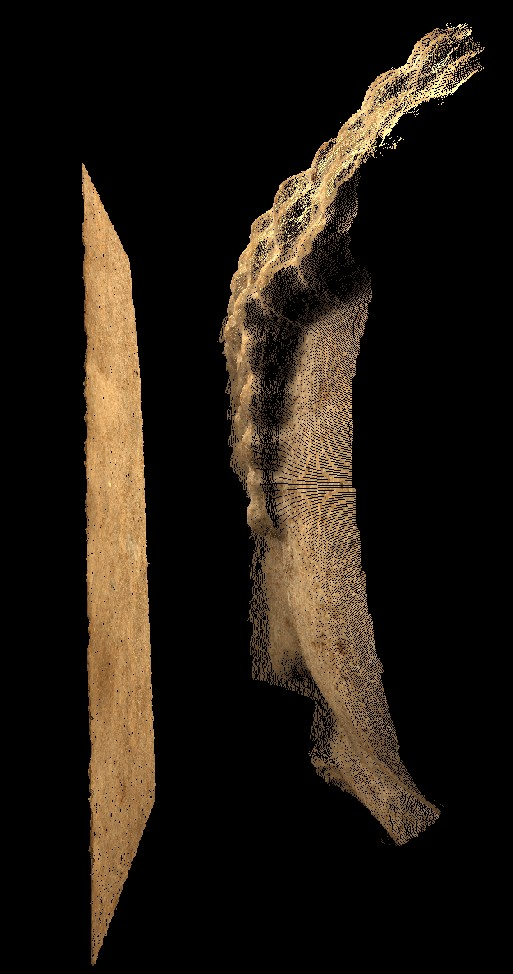
\includegraphics[height=55mm]{FIGS/Boudhas/Clou-5564.jpg}
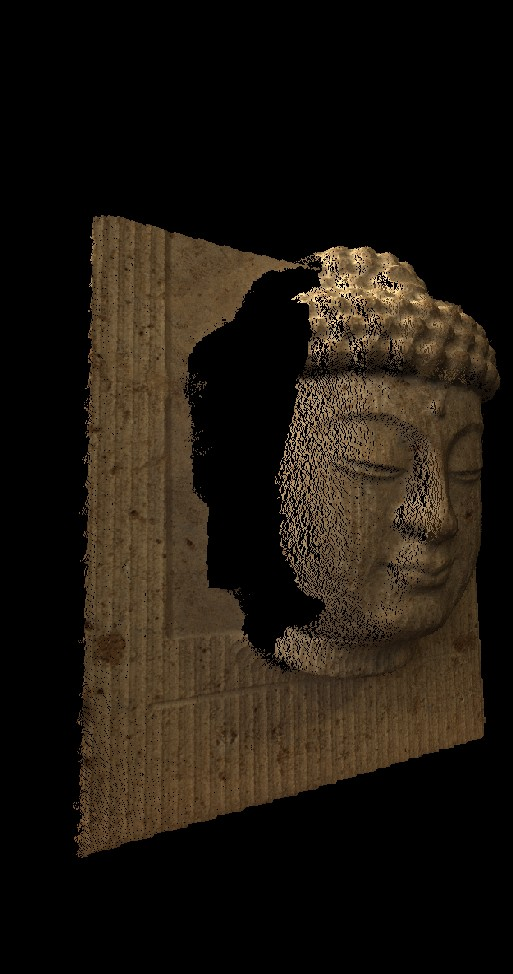
\includegraphics[height=55mm]{FIGS/Boudhas/Clou-5586.jpg}
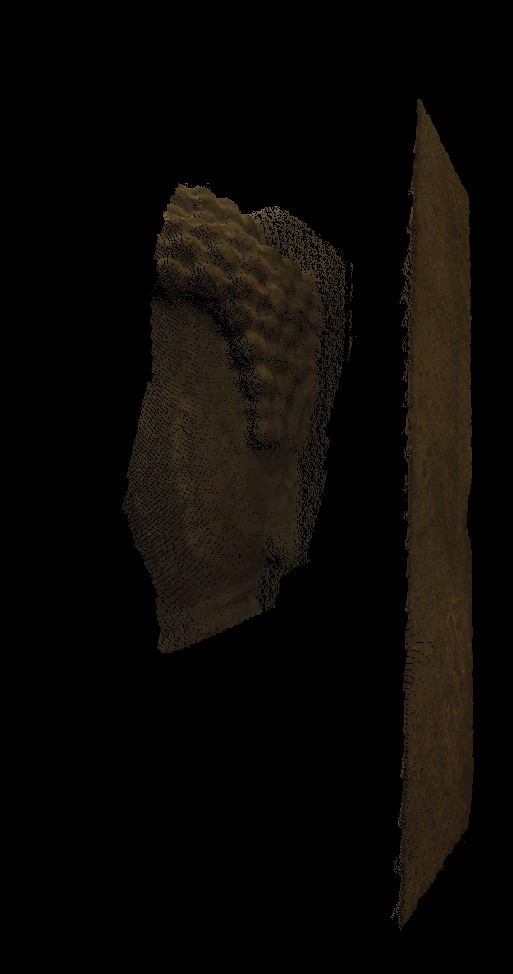
\includegraphics[height=55mm]{FIGS/Boudhas/Clou-5581.jpg}
\caption{The $3$ separate point clouds}
\label{BOUDHA:CLOUD:OUTPUT:SEP}
\end{center}
\end{figure}


\begin{figure}
\begin{center}
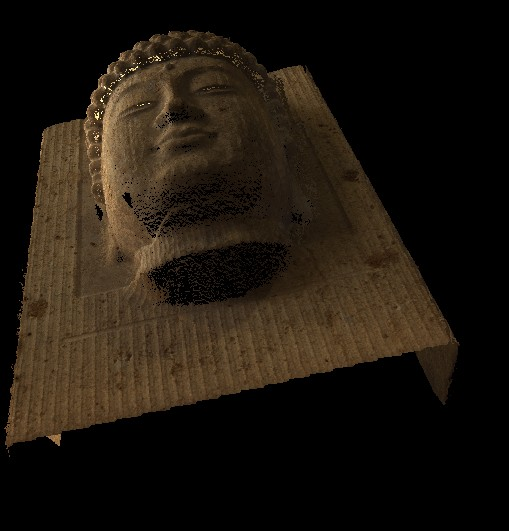
\includegraphics[height=55mm]{FIGS/Boudhas/PL-F2-A.jpg}
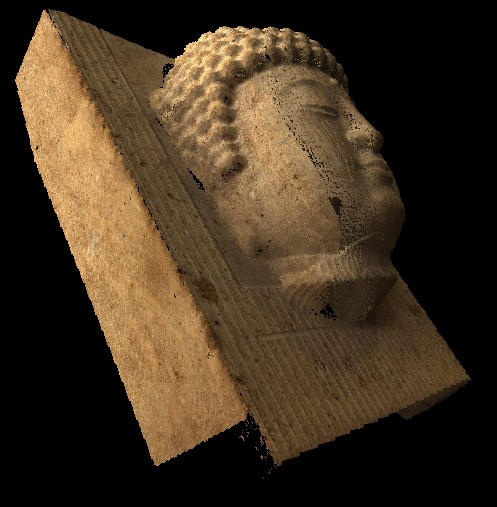
\includegraphics[height=55mm]{FIGS/Boudhas/PL-F2-B.jpg}
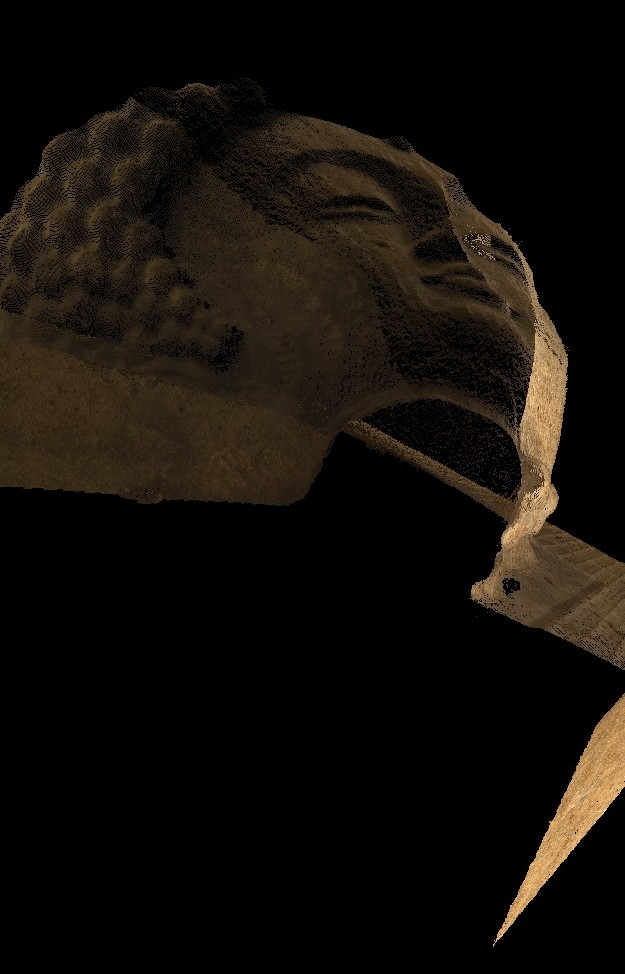
\includegraphics[height=55mm]{FIGS/Boudhas/PL-F2-C.jpg}
\caption{Some views of the merged point cloud}
\label{BOUDHA:CLOUD:OUTPUT:MERGE}
\end{center}
\end{figure}

%-------------------------------------------------------------------
%-------------------------------------------------------------------
%-------------------------------------------------------------------

\section{Hidden part and individual ortho images generation}


In the curent version of {\tt MicMac},  the formula used for multi-correlation is
by default  the average of cross correlation on all pair of images (see~\ref{Multi:Correl:Coef}
for variants).  When there are  part of the ground that are not seen on some images,
it would be more appropriate to compute the average on the only image that see some
part of the ground. We can compute hidden part if we know a $3D$ model of the scene.
Obviously, we don't have a "perfect" $3d$ models~\footnote{else, we would not loose our
time to make work irritating correlation tools \dots } but with multi-resolution
approach, there are case where the solution of previous steps may be an acceptable
approximation of the 3D for hidden part computation.
The file {\tt Param-7-Ter.xml} gives an example of how this functionnality
can be used in {\tt MicMac}  :


{\scriptsize
\begin{verbatim}
...
        <EtapeMEC>
                 <DeZoom >        8        </DeZoom>
        </EtapeMEC>
        <EtapeMEC>
                 <DeZoom >        4        </DeZoom>
                 <GenerePartiesCachees >
                       <ByMkF> true </ByMkF>
                       <SeuilUsePC> 3 </SeuilUsePC>
                </GenerePartiesCachees>
        </EtapeMEC>
        <EtapeMEC>
                 <DeZoom>        2        </DeZoom>
                 <GenerePartiesCachees >
                       <ByMkF> true </ByMkF>
                       <SeuilUsePC> 3 </SeuilUsePC>
                </GenerePartiesCachees>
        </EtapeMEC>
...     
\end{verbatim}
}


At resolution $4$ and $2$, there is a {\tt <GenerePartiesCachees>}, when this tag
is encontered, {\tt MicMac} will compute \footnote{using a classical Z-buffer algorithm}
at the end of the processing
step , for each of the input image, an image
superposable to the DTM; this image indicates for each pixel if this pixel is visible
or hidden. For example, you can see in directory {\tt MEC-7-Ter}, that 
a file {\tt  MasqPC\_LeChantier\_Num2\_IMG\_5588.tif} has been created.

As the DTM is not perfect,  if the result is used without further precaution, 
every small noise inside it, can cause a small hidden part in the computation.
The two right image of figure~\ref{Hidden:part} show the mask that would
result from a direct use of hidden part : there would be everywhere in
the image a lot of isolated pixels supposed to be hiddden; 

In fact the notion of hidden part, is not a binary notion, intutitevely it's
easy to understand that some points are weakly hidden do a relief of a few pixels,
and that others are strongly hidden by high reliefs. MicMac compute a value
that implement this intuitive notion, third image of figure~\ref{Hidden:part}
presents in gray level such a quantitative notion of hidden part.
We can now describe the subtags of {\tt <GenerePartiesCachees>} :


\begin{itemize}
   \item  {\tt  <SeuilUsePC>} is used to  threshold the quantitative hidden
          image that has been computed by MicMac; points over this threshold
          will not be used in the correlation computation; fourth image of
          figure~\ref{Hidden:part} present the thresholded image;
   \item  {\tt  <ByMkF>} just mean that you allow MicMac to parallelize the 
          computation (in fact should alway be true except for debuging);
\end{itemize}


\begin{figure}
\begin{tabular}{||c|c|c|c||}
   \hline \hline
   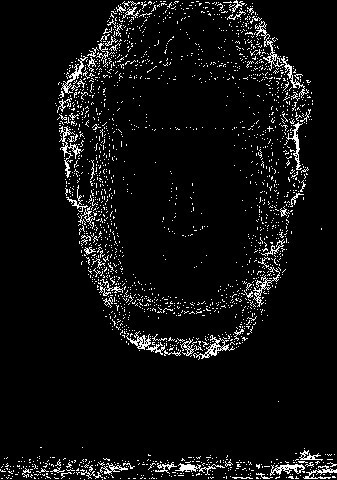
\includegraphics[width=40mm]{FIGS/Boudhas/MASQ_BRUTE_5588.jpg}  &
   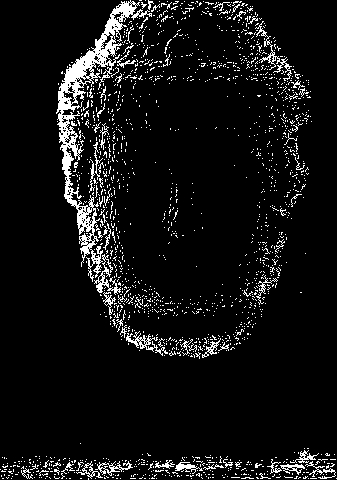
\includegraphics[width=40mm]{FIGS/Boudhas/MASQ_BRUTE_5592.jpg}  &
   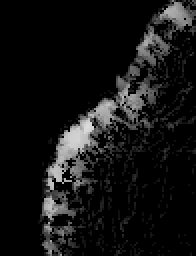
\includegraphics[width=40mm]{FIGS/Boudhas/MASQ_GRAY_5592.jpg}  &
   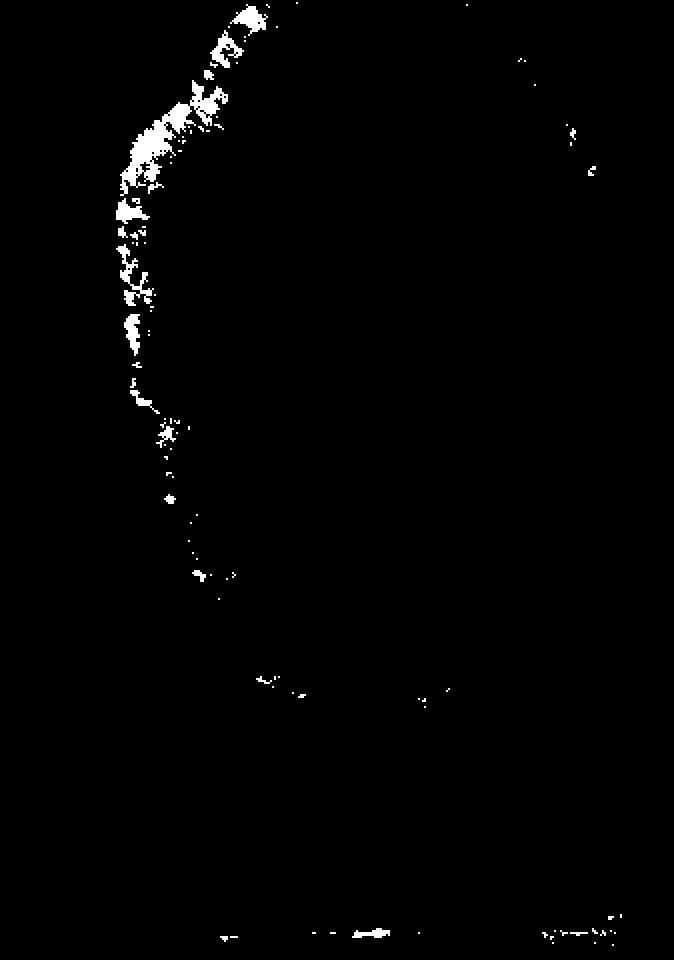
\includegraphics[width=40mm]{FIGS/Boudhas/MASQ_SEUIl_5592.jpg}  \\ \hline  \hline
\end{tabular}
\label{Hidden:part}
\caption{Images 1 et 2 : exemple of binary hidden part; Image 3 , gray funtction of hidden part; Image 4 : thesholded
hidden part function }
\end{figure}


While {\tt MicMac} is computing the hidden part, he has in fact almost all the information
necessary  to compute the geometric deformation necessary to make ortho-images. This why
the tag {\tt <MakeOrthoParImage>} allowing this ortho computation is a sub-tag of
 {\tt GenerePartiesCachees>}:

{\scriptsize
\begin{verbatim}
        <EtapeMEC>
                 <DeZoom >        1        </DeZoom>
                 <GenerePartiesCachees >
                       <ByMkF> true </ByMkF>
                       <SeuilUsePC> 3 </SeuilUsePC>
                       <KeyCalcPC> NKS-Assoc-AddDirAndPref@ORTHO@PC_ </KeyCalcPC>
                       <MakeOrthoParImage >
                           <KeyCalcInput>    Key-Assoc-Id </KeyCalcInput>
                           <KeyCalcOutput >  NKS-Assoc-AddDirAndPref@ORTHO@Ort_ </KeyCalcOutput>
                           <KeyCalcIncidHor> NKS-Assoc-AddDirAndPref@ORTHO@Incid_ </KeyCalcIncidHor>
                           <!-- Par rapport a la resolution des image R1 -->
                           <ResolIm> 1.0 </ResolIm>
                           <CalcIncAZMoy> true </CalcIncAZMoy>
                       </MakeOrthoParImage>
                </GenerePartiesCachees>
        </EtapeMEC>

\end{verbatim}
}

Some comments on this  part of the file :

\begin{itemize}
    \item  this is made at a final step of the computation, so the hidden part will not be reused in correlation,
           however they are computed because they are usefull for mosaincing (see~\ref{Porto}).

    \item the input image to ortho-rectify is specified by {\tt <KeyCalcInput>}; here it is the same
          image that the correlation image, so we use the special key {\tt Key-Assoc-Id};

    \item {\tt NKS-Assoc-AddDirAndPref} is a parametrized key that generate name under a different directory
          and add pref (see the definition in {\tt DefautChantierDescripteur.xml}); it used several time
          because we need to general several file for each image;
 

    \item the generated files  are :

    \begin{itemize}
            \item the individual ortho image, its name is specified by {\tt <KeyCalcOutput>};
            \item the hidden part image specified by {\tt <KeyCalcPC>};
            \item the incidence image  specified by {\tt <KeyCalcIncidHor>}; this image we be used
                  in mosaicing to select, between the different individual ortho-image, which is
                  the best (i.e. incident ray is closest to vertical);
    \end{itemize}

\end{itemize}

The figure ~\ref{Resul:Ortho:MM} present the input and ouput of this ortho-image generation.

\begin{figure}
\begin{tabular}{||c|c|c|c||}
   \hline \hline
   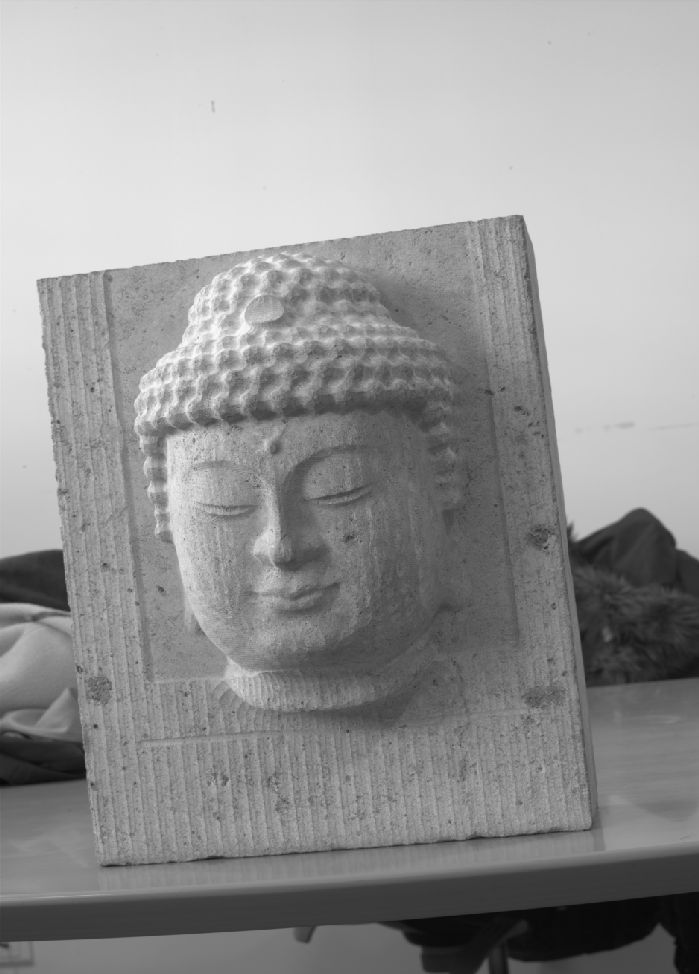
\includegraphics[width=40mm]{FIGS/Boudhas/IMG_5592.jpg} &
   
\includegraphics[width=40mm]{FIGS/Boudhas/Incid_IMG_5592_8Bits.jpg} &
   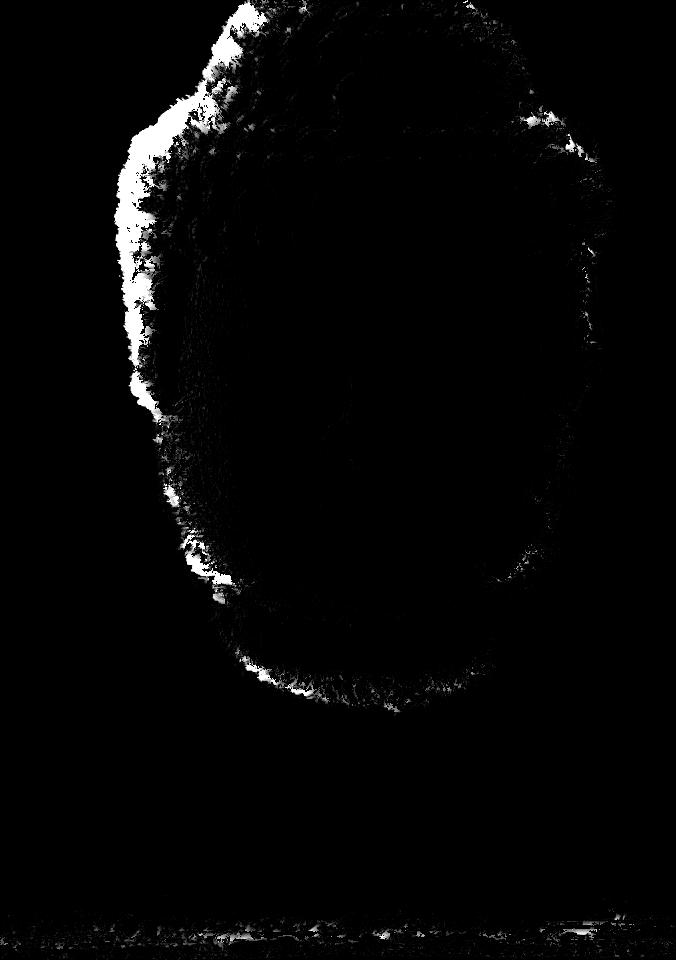
\includegraphics[width=40mm]{FIGS/Boudhas/Hidden_5592.jpg}  &
   \includegraphics[width=40mm]{FIGS/Boudhas/Ort_IMG_5592.jpg} \\ \hline  \hline
\end{tabular}
\label{Resul:Ortho:MM}
\caption{An image (5592) and the results of individual ortho generation: 
its incidence image, its hidden part image, its single ortho-image}
\end{figure}












%-------------------------------------------------------------------
\subsection{Other Options}
%-------------------------------------------------------------------
%-------------------------------------------------------------------
%-------------------------------------------------------------------

\section{2D Matching}

This section will describe the possibility offered when the orientations
are unprecise and the matching needs to be 2-dimensional.

\subsection{Pure Image 2D Matching}
Epipolare bi-dim avec Boudah

\subsection{Ground Image 2D Matching}

%-------------------------------------------------------------------
%-------------------------------------------------------------------
%-------------------------------------------------------------------
 




